%%%%%%%%%%%%%%%%%%%%%%%%%%%%%%%%%%%%%%%%%
% Beamer Presentation
% LaTeX Template
% Version 1.0 (10/11/12)
%
% This template has been downloaded from:
% http://www.LaTeXTemplates.com
%
% License:
% CC BY-NC-SA 3.0 (http://creativecommons.org/licenses/by-nc-sa/3.0/)
%
%%%%%%%%%%%%%%%%%%%%%%%%%%%%%%%%%%%%%%%%%

%----------------------------------------------------------------------------------------
%	PACKAGES AND THEMES
%----------------------------------------------------------------------------------------

%%%%\documentclass[aspectratio=169]{beamer}
%%%%%%\documentclass{beamer}
%%%%\mode<presentation> {
%%%%
%%%%% The Beamer class comes with a number of default slide themes
%%%%% which change the colors and layouts of slides. Below this is a list
%%%%% of all the themes, uncomment each in turn to see what they look like.
%%%%
%%%%%\usetheme{default}
%%%%%\usetheme{AnnArbor}
%%%%%\usetheme{Antibes}
%%%%%\usetheme{Bergen}
%%%%%\usetheme{Berkeley}
%%%%%\usetheme{Berlin}
%%%%%\usetheme{Boadilla}
%%%%%\usetheme{CambridgeUS}
%%%%%\usetheme{Copenhagen}
%%%%%\usetheme{Darmstadt}
%%%%%\usetheme{Dresden}
%%%%%\usetheme{Frankfurt}
%%%%%\usetheme{Goettingen}
%%%%%\usetheme{Hannover}
%%%%%\usetheme{Ilmenau}
%%%%%\usetheme{JuanLesPins}
%%%%%\usetheme{Luebeck}
%%%%\usetheme{Madrid}
%%%%%\usetheme{Malmoe}
%%%%%\usetheme{Marburg}
%%%%%\usetheme{Montpellier}
%%%%%\usetheme{PaloAlto}
%%%%%\usetheme{Pittsburgh}
%%%%%\usetheme{Rochester}
%%%%%\usetheme{Singapore}
%%%%%\usetheme{Szeged}
%%%%%\usetheme{Warsaw}
%%%%
%%%%% As well as themes, the Beamer class has a number of color themes
%%%%% for any slide theme. Uncomment each of these in turn to see how it
%%%%% changes the colors of your current slide theme.
%%%%
%%%%%\usecolortheme{albatross}
%%%%%\usecolortheme{beaver}
%%%%%\usecolortheme{beetle}
%%%%%\usecolortheme{crane}
%%%%%\usecolortheme{dolphin}
%%%%%\usecolortheme{dove}
%%%%%\usecolortheme{fly}
%%%%%\usecolortheme{lily}
%%%%%\usecolortheme{orchid}
%%%%%\usecolortheme{rose}
%%%%%\usecolortheme{seagull}
%%%%%\usecolortheme{seahorse}
%%%%%\usecolortheme{whale}
%%%%%\usecolortheme{wolverine}
%%%%
%%%%%\setbeamertemplate{footline} % To remove the footer line in all slides uncomment this line
%%%%%\setbeamertemplate{footline}[page number] % To replace the footer line in all slides with a simple slide count uncomment this line
%%%%
%%%%%\setbeamertemplate{navigation symbols}{} % To remove the navigation symbols from the bottom of all slides uncomment this line
%%%%}
%%%%%%\documentclass[mathserif,hyperref={pdfpagemode=FullScreen}]{beamer}
%%%%%%% \documentclass[handout]{beamer}
%%%%%%% \usetheme{Dresden}
%%%%%%\usetheme{340}
%%%%%%\beamertemplatetransparentcovereddynamic
%%%%%%\usepackage[latin1]{inputenc}
%%%%%%\usepackage{pgf}

\documentclass[mathserif,hyperref={pdfpagemode=FullScreen}]{beamer}
% \documentclass[handout]{beamer}
% \usetheme{Dresden}
\usetheme{340}
\beamertemplatetransparentcovereddynamic
\usepackage[latin1]{inputenc}
\usepackage{pgf}


\usepackage{amsmath,amsfonts,amssymb}
\usepackage{xspace}
%%\usepackage{algorithm}
\usepackage{algorithmic}
\usepackage{xcolor}
\usepackage{graphicx} % Allows including images
\usepackage{booktabs} % Allows the use of \toprule, \midrule and \bottomrule in tables
%%\usepackage{xspace}

\usepackage{braket}


\newcommand{\heteroprio}{{HeteroPrio}\xspace}
\newcommand{\heteroprioD}{{HeteroPrioDep}\xspace}


%%\usepackage{tcolorbox}
\usepackage{tikz}
\usetikzlibrary{matrix, decorations, patterns, positioning, shapes, calc, intersections, arrows, fit}


\usetikzlibrary{patterns}
\usetikzlibrary{fit,calc,positioning,decorations.pathreplacing,matrix}
%%\tikzset{xtick/.style={inner xsep=0pt, inner ysep=3pt, minimum
%%		size=0pt, draw, label=below:#1},%
%%	comm/.style args={#1start#2length#3color#4}{rounded corners=1mm, draw, inner
%%		sep=0pt, fill=#4, label=center:#1, fit={(#2,0.75)
%%			(#2+#3,1.5)}},%
%%	comp/.style args={#1start#2length#3color#4}{rounded corners=1mm, draw, inner
%%		sep=0pt, fill=#4, label=center:#1, fit={(#2,0)
%%			(#2+#3,0.75)}},%
%%}
%%
%%\newcommand{\schedule}[3]{
%%	\draw[->] (-0.2, 0) -- (#1, 0) node[below] {$t$};
%%	\draw (0, 0) -- (0, 1.5);
%%	\node at (-0.8, 0.75)[rotate=90] {#2};
%%	\draw[dashed,gray] (0, 0.75) -- (#1, 0.75);
%%	\foreach \t in {0,#3} {
%%		\node[xtick=\t] at (\t, 0){};
%%	}
%%}
%%\newcommand{\task}[6][0]{
%%	\node[comm=#2 start #3 length #4 color #6]{};
%%	\node[comp=#2 start #3+#4+#1 length #5 color #6]{}; 
%%}


\newcommand\addvmargin[1]{
	\node[fit=(current bounding box),inner ysep=#1,inner xsep=0]{};
}

\newcommand{\tensor}[1]{{\cal\textbf{#1}\xspace}}
\newcommand{\ttrain}{{\it Tensor-Train}\xspace}

\newcommand{\hfirst}{{\it LSR}\xspace}
\newcommand{\hsecond}{{\it SLSB}\xspace}
\newcommand{\hthird}{{\it LSB}\xspace}
\newcommand{\otta}{{\it STTA}\xspace}


\newcommand{\credit}[1]{\vspace*{-0.2cm}\par\hfill {\footnotesize Source:~\itshape#1}}



%% Colors from https://latexcolor.com/
\definecolor{pastelviolet}{rgb}{0.8, 0.6, 0.79}
\definecolor{babyblueeyes}{rgb}{0.63, 0.79, 0.95}
\definecolor{pastelyellow}{rgb}{0.99, 0.99, 0.59}
\definecolor{pastelgreen}{rgb}{0.47, 0.87, 0.47}
\definecolor{pastelred}{rgb}{1.0, 0.41, 0.38}
\colorlet{patternblue}{blue!60}


\definecolor{forestgreen}{rgb}{0.13, 0.55, 0.13}
\definecolor{greenhtml}{rgb}{0.0, 0.5, 0.0}
\definecolor{cyannew}{rgb}{0.0, 1.0, 1.0}




%----------------------------------------------------------------------------------------
%	TITLE PAGE
%----------------------------------------------------------------------------------------

\newcommand{\ignore}[1]{}
 
\usepackage{color}
\usepackage{subfigure}
\usepackage{colortbl}
\usepackage{epsfig}
\usepackage{verbatim}
\usepackage{array}
\usepackage{fancybox}
\usepackage{longtable}
\usepackage{epic,eepic}
%%\usepackage{algorithmic} 
%\usepackage{algorithmic2}   % for Lyon's algo format
%\usepackage{algorithm}
\usepackage{xspace} 
\usepackage{psfrag}         % for modifying figures
\usepackage{wasysym}        % for smileys
\usepackage{amsmath,amsthm,amssymb,subfigure}
\usepackage{times}
\usepackage{url}
\usepackage[boxed,vlined]{algorithm2e}
\usepackage{wasysym}        % for smileys                              


\newcommand{\VIO}[1]{\ifthenelse{\equal{#1}{}}{\ensuremath{V^{I/O}}\xspace}{\ensuremath{V^{I/O}_{#1}}\xspace}}


%%%%%% MIN_IO
\newcommand{\mat}[1]{{\small \tt #1}}
\newcommand{\order}[1]{{\small \tt #1}}
\newcommand{\soft}[1]{{\tt #1}}
\newcommand{\MinMem}{{\tt MinMEM}\xspace}
\newcommand{\MinMembf}{{\small \bf MinMEM}\xspace}
\newcommand{\MinIO}{{\tt MinIO}\xspace}
\newcommand{\MinIObf}{{\small \bf MinIO}\xspace}
\newcommand{\inplace}{{\emph{in-place}}\xspace}
\newcommand{\maxcbinplace}{{\emph{max-in-place}}\xspace}
\newcommand{\lastcbinplace}{{\emph{last-in-place}}\xspace}
\newcommand{\classical}{{\emph{classical}}\xspace}
\newcommand{\Maxcbinplace}{{\emph{Max-in-place}}\xspace}
\newcommand{\Lastcbinplace}{{\emph{Last-in-place}}\xspace}
\newcommand{\Classical}{{\emph{Classical}}\xspace}

%%%%%% Cite beamer
\newcommand{\citefull}[2]{{\footnotesize {\tt #1} '{$#2$}}}

%%%%% Colors
\newcommand<>{\blue}[1]{{\color#2{blue!100!black!100}#1}}
\newcommand<>{\green}[1]{{\color#2{green!100!black!100}#1}}
\newcommand<>{\red}[1]{{\color#2{red!100!black!100}#1}}

%%%%% Theorems
\newtheorem{myprop}{Property}
\newtheorem{mydef}{Definition}



%smileys % green - red
\def\smiley{\green{\wasyfamily\char44}\xspace}
\def\frownie{\red{\wasyfamily\char47}\xspace}

%%% OOC %%%
\newcommand{\IO}{\emph{I/O}\xspace}
\newcommand{\IOs}{\IO{}s\xspace}
\newcommand{\Vmin}{{V_{\IO}}_{min}}
\newcommand{\ic}{{in-core}\xspace}
\newcommand{\ooc}{{out-of-core}\xspace}
\newcommand{\AllCB}{{\tt All-CB}\xspace}
\newcommand{\OneCB}{{\tt One-CB}\xspace}
\newcommand{\OnlyF}{{\tt Pa\-rent-On\-ly}\xspace}

%%% FLEX %%%
\newtheorem{mytheorem}{Theorem}
\def\posfather{\ensuremath{p}\xspace}
\def\nbchildren#1{\ensuremath{n}\xspace}
\def\i2p{\ensuremath{\mathcal{I}_{2P}}\xspace}
\def\imm{\ensuremath{\mathcal{I}_{TMM}}\xspace}
\def\mbold{\mathversion{bold}}
\def\mnorm{\mathversion{normal}}
\def\OPT#1{{\mbold\textsc{#1}}\xspace}
\newcommand{\class}{\textit{classic}}
\newcommand{\flex}{\textit{flex}}
\newcommand{\ant}{\textit{early}}
\newcommand{\classip}{\textit{class\_ip}}
\newcommand{\flexip}{\textit{flex\_ip}}
\newcommand{\antip}{\textit{early\_ip}}
\newcommand{\T}[2]{\ifthenelse{\equal{#1}{}}{\ensuremath{T^{#2}}\xspace}{
\ensuremath{T^{#2}_{#1}}\xspace}}
\newcommand{\M}[1]{\ifthenelse{\equal{#1}{}}{\ensuremath{M}\xspace}{\ensu
remath{M_{#1}}\xspace}}
\newcommand{\cb}[1]{\ifthenelse{\equal{#1}{}}{\ensuremath{\textit{cb}}\xs
pace}{\ensuremath{\textit{cb}_{#1}}\xspace}}
\newcommand{\factor}[1]{\ifthenelse{\equal{#1}{}}{\ensuremath{F}\xspace}{
\ensuremath{F_{#1}}\xspace}}
\newcommand{\child}[2]{\ensuremath{#2}\xspace}
\newcommand{\storage}[1]{\ensuremath{m}\xspace}
\newcommand{\storageforcearg}[1]{\ensuremath{m_{#1}}\xspace}
\renewcommand{\thesubfigure}{}


% Empeche les num�rotations des subfigure
\renewcommand{\thesubfigure}{}


\newcommand{\psfragSimul}{
\psfrag{Number of processors}{{\footnotesize Number of processors}}%
\psfrag{Memory peak (millions of reals)}{{\footnotesize Memory peak (millions of reals)}}%
\psfrag{Total memory}{\hspace{-.1cm}{\footnotesize Total memory}}%
\psfrag{Active memory}{{\footnotesize Stack \ic{}}}%
\psfrag{Pessimistic scheme}{\hspace{.05cm}{\footnotesize \AllCB{} scheme}}%
\psfrag{Intermediate scheme}{\hspace{.18cm}{\footnotesize \OneCB{} scheme}}%
\psfrag{Optimistic scheme}{\hspace{-1.05cm}{\footnotesize \OnlyF{}
    scheme}}%
}
\newcommand{\psfragFurther}{
\psfrag{Nombre de processeurs}{{\footnotesize Number of processors}}%
\psfrag{Saving (percentage)}{{\footnotesize Savings (percentage)}}%
\psfrag{In-core stack scheme}{\hspace{.70cm}{\footnotesize Stack \ic{}}}%
\psfrag{All-CB scheme}{\hspace{-.50cm}{\footnotesize \AllCB{} scheme}}%
\psfrag{One-CB scheme}{\hspace{-.30cm}{\footnotesize \OneCB{} scheme}}%
\psfrag{Parent-Only scheme}{\hspace{-.80cm}{\footnotesize
    \OnlyF{} scheme}}%
}


%%%%%%%% Matrices %%%%%%%%%%%%
\newcommand{\bbmat}{{\small \sc bbmat}}
\newcommand{\ecl}{{\small \sc ecl32}}
\newcommand{\extr}{{\small \sc invextr1}}
\newcommand{\fidap}{{\small \sc fidapm11}}
\newcommand{\garon}{{\small \sc garon2}}
\newcommand{\lhr}{{\small \sc lhr71c}}
\newcommand{\lnsp}{{\small \sc lnsp3937}}
\newcommand{\mix}{{\small \sc mixtank}}
\newcommand{\nasasrbrua}{{\footnotesize \sc nasasrb.rua}}
\newcommand{\nasasrb}{{\small \sc nasasrb}}
\newcommand{\rma}{{\small \sc rma10}}
\newcommand{\twotone}{{\small \sc twotone}}
\newcommand{\wangf}{{\small \sc wang4}}
% symmetric
\newcommand{\bmwcra}{{\small \sc bmwcra\_1}}
\newcommand{\bmwtrois}{{\small \sc bmw3\_2}}
\newcommand{\cranksegdeux}{{\small \sc cranksg2}}
\newcommand{\shiptroisrsa}{{\small \sc ship\_003.rsa}}
\newcommand{\shiptroisrse}{{\small \sc ship\_003.rse}}
\newcommand{\shiptrois}{{\small \sc ship\_003}}
\newcommand{\inline}{\small \sc inline\_1}

 
%%%%%%%% Snodal %%%%%%%%%%%%
\newcommand{\Forupto}[4]{
  \For{$#1 = #2 \; \mbox{\bf to}\; #3$}{#4}
}
\newcommand{\Foruptostep}[5]{
  \For{$#1 = #2 \; \mbox{\bf to}\; #3\; \mbox{\bf step}\; #4$}{#5}
}
\newcommand{\Fordownto}[4]{
  \For{$#1 = #2 \; \mbox{\bf downto}\; #3$}{#4}
}
\newcommand{\spcolor}{\color{blue} \footnotesize}

\newcommand{\pmf}{{\em multifrontal}\xspace}% pure multifrontal
\newcommand{\prl}{{\em right-looking}\xspace}% pure right-looking
\newcommand{\pll}{{\em left-looking}\xspace}% pure left-looking
\newcommand{\Pmf}{{\em Multifrontal}\xspace}% pure multifronal
\newcommand{\Prl}{{\em Right-looking}\xspace}% pure right-looking
\newcommand{\Pll}{{\em Left-looking}\xspace}% pure left-looking
\newcommand{\llrl}{{\em left-looking/right-looking}\xspace}% left/right
\newcommand{\llll}{{\em left-looking/left-looking}\xspace}% left/left
\newcommand{\rlrl}{{\em right-looking/right-looking}\xspace}% right/right
\newcommand{\rlll}{{\em right-looking/left-looking}\xspace}% right/left
\newcommand{\Llrl}{{\em Left-looking/right-looking}\xspace}% left/right
\newcommand{\Llll}{{\em Left-looking/left-looking}\xspace}% left/left
\newcommand{\Rlrl}{{\em Right-looking/right-looking}\xspace}% right/right
\newcommand{\Rlll}{{\em Right-looking/left-looking}\xspace}% right/left
\newcommand{\LLRL}{{\tt LL-RL}\xspace}
\newcommand{\LLLL}{{\tt LL-LL}\xspace}
\newcommand{\RLRL}{{\tt RL-RL}\xspace}
\newcommand{\RLLL}{{\tt RL-LL}\xspace}
\newcommand{\RL}{{\tt RL}\xspace}
\newcommand{\LL}{{\tt LL}\xspace}
\newcommand{\scgt}{{\em scatter/gather}\xspace}
\newcommand{\WORZ}{{\tt W1/R0}\xspace}
\newcommand{\WORO}{{\tt W1/R1}\xspace}
\newcommand{\WORM}{{\tt W1/RM}\xspace}
\newcommand{\WMRM}{{\tt WM/RM}\xspace}
\newcommand{\outterancestor}{{\emph{outer ancestor}}\xspace}
\newcommand{\outterancestors}{{\emph{outer ancestors}}\xspace}
\newcommand{\Outterancestor}{{\emph{Outer ancestor}}\xspace}
\newcommand{\Outterancestors}{{\emph{Outer ancestors}}\xspace}
\newcommand{\outersubtree}{{\emph{outer subtree}}\xspace}
\newcommand{\outersubtrees}{{\emph{outer subtrees}}\xspace}
\newcommand{\Outersubtree}{{\emph{Outer subtree}}\xspace}
\newcommand{\Outersubtrees}{{\emph{Outer subtrees}}\xspace}

\newcommand{\node}[1]{{\footnotesize \ensuremath{{\mathcal
        N}_{#1}}}\xspace}
\newcommand{\nodeps}[1]{{\tiny \ensuremath{{\mathcal N}_{#1}}}\xspace}
\newcommand{\subtree}[1]{{\ensuremath{S_{#1}}}\xspace}
\newcommand{\etree}{{\ensuremath{\textit{etree}}}\xspace}
\newcommand{\SET}{{\footnotesize \ensuremath{{\mathcal
        S}}}\xspace}
\newcommand{\SUBSET}{{\footnotesize \ensuremath{{\mathcal
        S}_{0}}}\xspace}
\newcommand{\nodeSET}[1]{{\ensuremath{s_{#1}}}\xspace}
\newcommand{\TOTSET}{{\footnotesize \ensuremath{{S}}}\xspace}
\newcommand{\XSET}{{\footnotesize \ensuremath{{\mathcal
        X}}}\xspace}
\newcommand{\XSUBSET}{{\footnotesize \ensuremath{{\mathcal
        X}_{0}}}\xspace}
\newcommand{\nodexSET}[1]{{\ensuremath{x_{#1}}}\xspace}
\newcommand{\TOTXSET}{{\footnotesize \ensuremath{{X}}}\xspace}

\newcommand{\psfragnumbering}{
        \psfrag{2}{{2}}\psfrag{3}{{3}}\psfrag{4}{{4}}
        \psfrag{5}{{5}}\psfrag{6}{{6}}\psfrag{7}{{7}}\psfrag{8}{{8}}
        \psfrag{9}{{9}}\psfrag{10}{{10}}\psfrag{11}{{11}}\psfrag{12}{{12}}
        \psfrag{13}{{13}}\psfrag{14}{{14}}\psfrag{15}{{15}}
}

\newcommand{\psfragnumberingcolored}{
        \psfrag{1}{{\spcolor 1}}
        \psfrag{2}{{\spcolor 2}}\psfrag{3}{{\spcolor 3}}
        \psfrag{4}{{\spcolor 4}} \psfrag{5}{{\spcolor 5}}
}

\newcommand{\psfraglegend}{
    \psfrag{P}{{Node being processed}}%
    \psfrag{C}{{Nodes in memory}}%
    \psfrag{D}{{Node on disk}}%
    \psfrag{N}{{Node not yet loaded}}%
}
\newcommand{\psfragsubtrees}{
  \psfrag{S1}{{\footnotesize \subtree{1}}}
  \psfrag{S2}{{\footnotesize \subtree{2}}}
  \psfrag{S3}{{\footnotesize \subtree{3}}}
  \psfrag{S4}{{\footnotesize \subtree{4}}}
}
\newcommand{\psfraglocRL}{
        \psfrag{n1}{{\nodeps{1}}}\psfrag{n2}{{\nodeps{2}}}\psfrag{n3}{{\nodeps{3}}}
        \psfrag{S1}{{\subtree{1}}}\psfrag{S2}{{\subtree{2}}}
}
\newcommand{\psfraglocLL}{
  \psfragsubtrees
  \psfrag{SP}{{\SP}}
}
\newcommand{\psfragLLRL}{\psfragsubtrees} 
\newcommand{\psfragLLLL}{\psfragsubtrees} 
\newcommand{\psfraglegendLLRL}{
  \psfragsubtrees 
  \psfrag{SP}{{Current \SuperPanel}}
  \psfrag{S}{{Subtree}}
  \psfrag{US}{{Updating Subtree}}
} 
\newcommand{\psfraglegendLLRLtoLLLL}{
  \psfragsubtrees 
  \psfrag{SP}{{Focused subgraph}}
  \psfrag{S}{{Subtree}}
  \psfrag{US}{{Updating Subtree}}
} 
\newcommand{\psfraglegendLLLL}{
  \psfragsubtrees 
  \psfrag{SP}{{\SuperPanel}}
  \psfrag{CSP}{{\SuperPanel being processed}}
} 
\newcommand{\psfragreversibledchain}{
  \psfrag{3}{{\spcolor $3$}}
  \psfrag{5}{{\spcolor $5$}}
}
\newcommand{\psfragreversibledchainfullrlll}{
  \psfrag{Method}{{\RLLL}}
  \psfrag{4}{{\spcolor $4$}}
  \psfrag{1}{{\spcolor $1$}}
}
\newcommand{\psfragreversibledchainfullllrl}{
  \psfrag{Method}{{\LLRL}}
  \psfrag{7}{{\spcolor $7 \leq 4 + 4$}}
  \psfrag{0}{{\spcolor $0 \leq 1$}}
}
\newcommand{\psfragreversibledchainvio}{
  \psfrag{Method}{{}}
  \psfrag{4}{{\spcolor $4 \times 1$}}
  \psfrag{1}{{\spcolor $1 \times 2$}}
}
\newcommand{\psfragreversibledchainviollrl}{
  \psfrag{Method}{{}}
  \psfrag{6}{{\spcolor $6 \times 1$}}
  \psfrag{4}{{\spcolor $4 \times 2$}}
}
\newcommand{\psfragnodeSET}{
  \psfrag{S0}{{\nodeSET{0}}}
  \psfrag{S1}{{\nodeSET{1}}}
  \psfrag{S2}{{\nodeSET{2}}}
  \psfrag{S3}{{\nodeSET{3}}}
  \psfrag{S4}{{\nodeSET{4}}}
  \psfrag{S5}{{\nodeSET{5}}}
  \psfrag{S6}{{\nodeSET{6}}}
  \psfrag{Sn}{{\nodeSET{n}}}
}
\newcommand{\psfragsumSET}{
  \psfrag{S0}{{}}
  \psfrag{S1}{{\nodexSET{1}}}
  \psfrag{S2}{{\nodexSET{2}}}
  \psfrag{S3}{{\nodexSET{3}}}
  \psfrag{S4}{{\nodexSET{4}}}
  \psfrag{S5}{{\nodexSET{5}}}
  \psfrag{S6}{{\nodexSET{6}}}
  \psfrag{Sn}{{\nodexSET{n}}}
}
\newcommand{\psfragpeigne}{
  \psfrag{k}{{$k$}}
}

\newcommand{\SuperPanel}{{SuperPanel}\xspace}
\newcommand{\SuperPanels}{{SuperPanels}\xspace}
\newcommand{\HyperNode}{{HyperNode}\xspace}
\newcommand{\HyperNodes}{{HyperNodes}\xspace}
\newcommand{\SP}{{\ensuremath{\mbox{SP}}}\xspace}
\newcommand{\HN}{{\ensuremath{\mbox{HN}}}\xspace}
\newcommand{\SPA}{{\ensuremath{\mbox{SPA}}}\xspace}% Sparse Accumulator

\def\bydefn{\stackrel{def}{=}}
\def\comment#1{\textit{/*#1*/}}
\newcommand{\LU}{{${\bf L}{\bf U}$}}
\newcommand{\lu}{{${\bf L}{\bf U}$}}
\newcommand{\LDLT}{{${\bf L}{\bf D}{\bf L}^T$}}
\newcommand{\ldlt}{{${\bf L}{\bf D}{\bf L}^T$}}
\newcommand{\mumps}{{\tt MUMPS}\xspace}
\newcommand{\MUMPS}{{\tt MUMPS}\xspace}
\newcommand{\WinMUMPS}{{\tt WinMumps}\xspace}
%\newcommand{\PLASMA}{{\tt PLASMA}\xspace}
\newcommand{\MPI}{{\tt MPI}\xspace}
\newcommand{\OpenMP}{{\tt OpenMP}\xspace}
\newcommand{\MPICHV}{{\tt MPICH-V}\xspace}
\newcommand{\superlu}{{\tt SuperLU}\xspace}
\newcommand{\SuperLU}{{\tt SuperLU}\xspace}
\newcommand{\blas}{{\small \tt BLAS}\xspace}         
\newcommand{\CEACESTA}{{\sc Cea-Cesta}\xspace}
\newcommand{\AQUILON}{{\sc Aquilon}\xspace}
\newcommand{\fantome}{\phantom{0}}
\newcommand{\NP}{{NP-complete}}
\newcommand{\NPess}{{NP-completeness}}
\newcommand{\panelizellll}{{Panelize-LL-LL}}
\newcommand{\panelizellllopt}{{Panelize-LL-LL-OPT}}
\newcommand{\panelizelllldec}{{Panelize-LL-LL-DEC}}
\newcommand{\maximumsubsetsum}{{Maximum-Subset-Sum}}


\newtheorem{proposition}{Proposition}
\newtheorem{property}{Property}
\newtheorem{assumedef}{Assumption}


%%%  LARGE_PBS  %%%
\newcommand{\Store}[1]{\ifthenelse{\equal{#1}{}}{\ensuremath{S}\xspace}{\ensuremath{S_{#1}}\xspace}}
\newcommand{\EffMemMax}{{\ensuremath{e}}\xspace}
\newcommand{\EffMemAvg}{{\ensuremath{e_{avg}}}\xspace}
\newcommand{\work}[1]{\ifthenelse{\equal{#1}{}}{\ensuremath{W}\xspace}{\ensuremath{W_{#1}}\xspace}}


%%% PLASMA %%%
\newcommand{\MAGMA}{{\tt MAGMA}\xspace}
\newcommand{\PLASMA}{{\tt PLASMA}\xspace}
\newcommand{\TBLAS}{{\tt TBLAS}\xspace}
\newcommand{\PESSL}{{\tt PESSL}\xspace}
\newcommand{\ESSL}{{\tt ESSL}\xspace}
\newcommand{\MKL}{{\tt MKL}\xspace}
\newcommand{\SCALAPACK}{{\tt SCALAPACK}\xspace}
\newcommand{\LAPACK}{{\tt LAPACK}\xspace}
\newcommand{\DPOTRF}{{\tt DPOTRF}\xspace}
\newcommand{\DGEQRF}{{\tt DGEQRF}\xspace}
\newcommand{\DGETRF}{{\tt DGETRF}\xspace}
\newcommand{\DGEMM}{{\tt DGEMM}\xspace}
\newcommand{\DGEMV}{{\tt DGEMV}\xspace}
\newcommand{\Intel}{{\tt Intel64}\xspace}
\newcommand{\Power}{{\tt Power6}\xspace}


%%% Smileys
\def\smiley{\green{\wasyfamily\char44}\xspace}
\def\frownie{\red{\wasyfamily\char47}\xspace}

% Add some command for name
\usepackage{xspace}
\newcommand{\linpack}{{\sc LinPACK}\xspace}
\newcommand{\lapack}{{\sc LAPACK}\xspace}
\newcommand{\scalapack}{{\sc ScaLAPACK}\xspace}
\newcommand{\pblas}{{\sc PBLAS}\xspace}
\newcommand{\plasma}{{\sc PLASMA}\xspace}
\newcommand{\magma}{{\sc MAGMA}\xspace}
\newcommand{\starpu}{{\sc StarPU}\xspace}
\newcommand{\goto}{{\sc GotoBLAS2}\xspace}
\newcommand{\gflops}{Gflop/s\xspace}
\newcommand{\mordor}{Opteron-Tesla\xspace}
\newcommand{\hannibal}{Nehalem-Quadro\xspace}


\newcommand{\kernel}[1]{\texttt{#1}\xspace}
%%\newcommand{\kernel}[1]{\emph{#1}\xspace}

\newcommand{\gemm}{\kernel{gemm}}
\newcommand{\sgemm}{\kernel{sgemm}}
\newcommand{\dgemm}{\kernel{dgemm}}
\newcommand{\trmm}{\kernel{trmm}}
\newcommand{\strmm}{\kernel{strmm}}
\newcommand{\dtrmm}{\kernel{dtrmm}}
\newcommand{\geqrt}{\kernel{geqrt}}
\newcommand{\sgeqrt}{\kernel{sgeqrt}}
\newcommand{\dgeqrt}{\kernel{dgeqrt}}
\newcommand{\ormqr}{\kernel{ormqr}}
\newcommand{\sormqr}{\kernel{sormqr}}
\newcommand{\dormqr}{\kernel{dormqr}}
\newcommand{\tsqrt}{\kernel{tsqrt}}
\newcommand{\stsqrt}{\kernel{stsqrt}}
\newcommand{\dtsqrt}{\kernel{dtsqrt}}
\newcommand{\tsmqr}{\kernel{tsmqr}}
\newcommand{\stsmqr}{\kernel{stsmqr}}
\newcommand{\dtsmqr}{\kernel{dtsmqr}}

\newcommand{\ttqrt}{\kernel{ttqrt}}
\newcommand{\ttmqr}{\kernel{ttmqr}}

\newcommand{\geqrf}{\kernel{geqrt}}
\newcommand{\sgeqrf}{\kernel{SGEQRF}}
\newcommand{\dgeqrf}{\kernel{DGEQRF}}

\AtBeginDocument{
	\title[Scalable Tensor Algorithms]{Scalable Tensor Algorithms for Modern Computing Systems}
		\author[{\sc Inria Paris}]{Suraj {\sc Kumar}\inst{1}}
	%%	\author[ICPP-2019]{\underline{Suraj {\sc Kumar}}\inst{1}, Lionel {\sc Eyraud-Dubois}\inst{2}, and\\ Sriram {\sc Krishnamoorthy}\inst{1}}
	\institute[shortinst]{\inst{1} Inria Paris, France}

}



%%\title[Scalable Tensor Algorithms]{Scalable Tensor Algorithms for Modern Computing Systems} % The short title appears at the bottom of every slide, the full title is only on the title page
%%
%%\author{Suraj {\sc Kumar}} % Your name
%%%%\institute[UCLA] % Your institution as it will appear on the bottom of every slide, may be shorthand to save space\institute[Inria Paris] % Your institution as it will appear on the bottom of every slide, may be shorthand to save space
%%%%{
%%%%	Alpines team, Inria Paris, France\\ % Your institution for the title page
%%%%	\medskip
%%%%	\textit{Suraj.kumar@inria.fr} % Your email address
%%%%}
%%%%{
%%%%University of California \\ % Your institution for the title page
%%%%\medskip
%%%%\textit{john@smith.com} % Your email address
%%%%}
%%\institute[Inria Paris] % Your institution as it will appear on the bottom of every slide, may be shorthand to save space
%%{
%%	Alpines team, Inria Paris, France\\ % Your institution for the title page
%%	\medskip
%%	\textit{Suraj.kumar@inria.fr} % Your email address
%%}
%%\date{\today} % Date, can be changed to a custom date



\makeatletter
\AtBeginPart{%
	\beamer@tocsectionnumber=0\relax
	\setcounter{section}{0}
	\frame{\partpage}%
}
\makeatother

\newcommand{\hiddencell}[2]{\action<#1->{#2}}
\begin{document}

\begin{frame}
\titlepage % Print the title page as the first slide
\end{frame}

\begin{frame}{Resume}
\begin{itemize}
	\item 11/2019 -- Current, Postdoc, Inria Paris, France
	\begin{itemize}
		\item Parallel algorithms for tensor computations, Use of tensors in  molecular simulations
	\end{itemize}
	\item 05/2018 -- 10/2019, Postdoc, Pacific Northwest National Laboratory, USA
	\begin{itemize}
		\item Theoretical and empirical analysis of data transfer orders, Task-based runtime systems for tensor operations of molecular simulations
	\end{itemize}
	\item 08/2017 -- 02/2018, Senior Engineer, Ericsson, Bangalore, India
	\begin{itemize}
		\item Use of remote GPUs in cloud
	\end{itemize}
	\item 12/2013 -- 06/2017, PhD Student, University of Bordeaux \& Inria Bordeaux, France
	\begin{itemize}
		\item Scheduling of dense linear algebra kernels on heterogeneous resources
	\end{itemize}
	\item 07/2012 -- 11/2013, Software Engineer, IBM Research, New Delhi, India
	\begin{itemize}
		\item Performance optimizations of TTI RTM algorithm on GPUs, Schedulers for BG/P machine
	\end{itemize}
	\item 08/2010 -- 06/2012, Master Student, Indian Institute of Science, Bangalore, India
	\begin{itemize}
		\item Automatic parallelization of programs with linked-list data structure 
	\end{itemize}
	\item 07/2006 -- 06/2010, BTech Student, Sikkim Manipal Institute of Technology, India
	\begin{itemize}
		\item Associating rule mining using genetic algorithm
	\end{itemize}
	
\end{itemize}
\end{frame}




\part[Past/Ongoing Work]{Past/Ongoing Work}

\begin{frame}{Collaborators}
This is joint work with ...
\begin{itemize}
	\item Laura Grigori -- Inria Paris, France
	\item Grey Ballard -- Wake Forest University, USA
	\item Hussam Al Daas -- STFC Rutherford Appleton Laboratory, UK
	\item Olivier Beaumont -- Inria Bordeaux, France
	\item Sriram Krishnamoorthy -- Pacific Northwest National Laboratory, USA
	\item Marcin Zalewski -- Nvidia, USA
	\item Lionel Eyraud-Dubois -- Inria Bordeaux, France
	\item Samuel Thibault -- Inria Bordeaux, France
	\item Emmanuel Agullo -- Inria Bordeaux, France
\end{itemize}
\end{frame}


\begin{frame}
\frametitle{Overview} % Table of contents slide, comment this block out to remove it
\tableofcontents[part=1] % Throughout your presentation, if you choose to use \section{} and \subsection{} commands, these will automatically be printed on this slide as an overview of your presentation
\end{frame}


\section{Tensors}

\begin{frame}{Tensors: Multidimensional Arrays}
\begin{tabular}{ccc}
	Dimension & Name &\\
	%%\begin{tikzpicture}[scale=0.625, every node/.style={transform shape}]
	%%\tikzstyle{taskr}=[draw=black, minimum height=1mm, minimum width=12mm, anchor=south west, fill=pastelgreen, text=black]
	%%			\node (t01) at (0,0) [taskr]{};
	%%\end{tikzpicture}
	%%\begin{tikzpicture}
	%%\pgfmathsetmacro{\cubex}{5}
	%%\pgfmathsetmacro{\cubey}{1}
	%%\pgfmathsetmacro{\cubez}{3}
	%%\draw[red,fill=yellow] (0,0,0) -- ++(-\cubex,0,0) -- ++(0,-\cubey,0) -- ++(\cubex,0,0) -- cycle;
	%%\draw[red,fill=yellow] (0,0,0) -- ++(0,0,-\cubez) -- ++(0,-\cubey,0) -- ++(0,0,\cubez) -- cycle;
	%%\draw[red,fill=yellow] (0,0,0) -- ++(-\cubex,0,0) -- ++(0,0,-\cubez) -- ++(\cubex,0,0) -- cycle;
	%%\end{tikzpicture}
	%%$0$ & Scalar & \\
	$1$ & Vector & 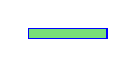
\begin{tikzpicture}[scale=0.25, every node/.style={transform shape}]
	\pgfmathsetmacro{\rectx}{4}
	\pgfmathsetmacro{\recty}{0.5}
	\draw[blue,fill=pastelgreen] (0,0) -- ++(-\rectx,0) -- ++(0,\recty) -- ++(\rectx, 0) -- cycle;
	\end{tikzpicture} \\
	&&\\
	$2$ & Matrix & 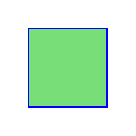
\begin{tikzpicture}[scale=0.25, every node/.style={transform shape}]
	\pgfmathsetmacro{\rectx}{4}
	\pgfmathsetmacro{\recty}{4}
	\draw[blue,fill=pastelgreen] (0,0) -- ++(-\rectx,0) -- ++(0,\recty) -- ++(\rectx, 0) -- cycle;
	%%\addvmargin{4};
	\end{tikzpicture}\\
	&&\\
	$3$ & $3$-dimensional tensor & 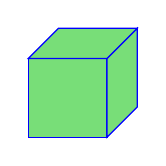
\begin{tikzpicture}[scale=0.25, every node/.style={transform shape}]
	\pgfmathsetmacro{\cubex}{4}
	\pgfmathsetmacro{\cubey}{4}
	\pgfmathsetmacro{\cubez}{4}
	\draw[blue,fill=pastelgreen] (0,0,0) -- ++(-\cubex,0,0) -- ++(0,-\cubey,0) -- ++(\cubex,0,0) -- cycle;
	\draw[blue,fill=pastelgreen] (0,0,0) -- ++(0,0,-\cubez) -- ++(0,-\cubey,0) -- ++(0,0,\cubez) -- cycle;
	\draw[blue,fill=pastelgreen] (0,0,0) -- ++(-\cubex,0,0) -- ++(0,0,-\cubez) -- ++(\cubex,0,0) -- cycle;
	\end{tikzpicture}\\
	&&\\
	$4$ & $4$-dimensional tensor & 
	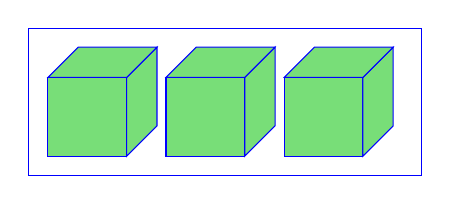
\begin{tikzpicture}[scale=0.25, every node/.style={transform shape}]
	\pgfmathsetmacro{\cubex}{4}
	\pgfmathsetmacro{\cubey}{4}
	\pgfmathsetmacro{\cubez}{4}
	\draw[blue,fill=pastelgreen] (0,0,0) -- ++(-\cubex,0,0) -- ++(0,-\cubey,0) -- ++(\cubex,0,0) -- cycle;
	\draw[blue,fill=pastelgreen] (0,0,0) -- ++(0,0,-\cubez) -- ++(0,-\cubey,0) -- ++(0,0,\cubez) -- cycle;
	\draw[blue,fill=pastelgreen] (0,0,0) -- ++(-\cubex,0,0) -- ++(0,0,-\cubez) -- ++(\cubex,0,0) -- cycle;
	
	\draw[blue,fill=pastelgreen] (\cubex +2,0,0) -- ++(-\cubex,0,0) -- ++(0,-\cubey,0) -- ++(\cubex,0,0) -- cycle;
	\draw[blue,fill=pastelgreen] (\cubex +2,0,0) -- ++(0,0,-\cubez) -- ++(0,-\cubey,0) -- ++(0,0,\cubez) -- cycle;
	\draw[blue,fill=pastelgreen] (\cubex +2,0,0) -- ++(-\cubex,0,0) -- ++(0,0,-\cubez) -- ++(\cubex,0,0) -- cycle;
	
	\draw[blue,fill=pastelgreen] (\cubex +2 + \cubex +2,0,0) -- ++(-\cubex,0,0) -- ++(0,-\cubey,0) -- ++(\cubex,0,0) -- cycle;
	\draw[blue,fill=pastelgreen] (\cubex +2 + \cubex +2,0,0) -- ++(0,0,-\cubez) -- ++(0,-\cubey,0) -- ++(0,0,\cubez) -- cycle;
	\draw[blue,fill=pastelgreen] (\cubex +2 + \cubex +2,0,0) -- ++(-\cubex,0,0) -- ++(0,0,-\cubez) -- ++(\cubex,0,0) -- cycle;
	
	\draw[blue, fill=none] (-\cubex -1, 2.5, 0) -- ++(0, -\cubey -3.5, 0) -- ++(\cubex +2 + \cubex +2 + \cubex + \cubex,0,0) -- ++(0, \cubey +3.5, 0) -- cycle; 
	\end{tikzpicture}
\end{tabular}

\end{frame}

%------------------------------------------------

%%\begin{frame}{Tensors}
%%\begin{itemize}
%%\item Tensors are used in several domains
%%\begin{itemize}
%%	\item Quantum molecular dynamics, signal processing, data mining, neurosciences, computer vision, psychometrics, chemometrics, ...
%%\end{itemize}
%%\vfill
%%\item Memory and computation requirements are exponential in the number of dimensions
%%\begin{itemize}
%%	\item A molecular simulation involving just $100$ spatial orbitals  manipulate a huge tensor with $4^{100}$ elements
%%	\item People work with low dimensional structure of the tensors
%%\end{itemize}
%%\vfill
%%\item Limited work on parallelization of tensor algorithms
%%%%    \begin{itemize}
%%%%    	\item Matricized Tensor Times Khatri Rao Product (MTTKRP), tensor contraction
%%%%    \end{itemize}
%%\end{itemize}
%%\end{frame}

\begin{frame}{Tensor Diagram Notations }
$Tensors are denoted by solid shapes aand number of lines coming out of the shapes denote the dimensions of the tensors.$

For example,
\includegraphics[scale=0.02]{./tmp/tensor-notation.jpg}

%%Tensors are notated by solid shapes, and tensor indices are notated by lines emanating from these shapes.
%%
%%Connecting two index lines implies a contraction, or summation over the connected indices

\begin{itemize}
	\item Connecting two lines implies summation over the connected dimensions
\end{itemize}
\end{frame}

\begin{frame}{Tensors are used in Several Domains}
\begin{itemize}
	\item \textbf{Neuroscience}: Neuron $\times$ Time $\times$ Trial
	\item \textbf{Transportation}: Pickup $\times$ Dropoff $\times$ Time
	\item \textbf{Media}: User x Movie x Time x Rating
	\item \textbf{Ecommerce}: User x Product x Rating
	\item \textbf{Cyber-Traffic}: IP x IP x Port x Time
	\item \textbf{Social-Network}: Person x Person x Time x Interaction-Type
\end{itemize}
\end{frame}

\begin{frame}{High Dimensional Tensors}
\begin{itemize}
	\item \textbf{Neural Network}:
	\includegraphics[scale=0.02]{./tmp/neuralNetwork.jpg}
	\item \textbf{Quantum or Molecular Simulation}:
	Approximation of $\psi$ in the Schrodinger equation, $\hat{H}\psi = E\psi$.
	$\hat{H}$ is an operator which corresponds to the total energy of the system. $\psi$ represents the quantum state of the system. It is a huge tensor with $2^n$ elements where $n$ is the number of electrons in the system or with $4^k$ elements where $k$ is the number of spatial orbitals in the consideration.
	
%%	\begin{align*}
%%	E&=\frac{\braket{\psi|H|\psi}}{\braket{\psi|\psi}}
%%	\end{align*}
	
%%	\item \textbf{PDEs with uncertain parameters}
\end{itemize}
\end{frame}


\begin{frame}{Tensors}
\begin{itemize}
%%	\item Tensors are used in several domains
%%	\begin{itemize}
%%		\item Quantum molecular dynamics, signal processing, data mining, neurosciences, computer vision, psychometrics, chemometrics, ...
%%	\end{itemize}
%%	\vfill
	\item Memory and computation requirements are exponential in the number of dimensions
	\begin{itemize}
		\item A molecular simulation involving just $100$ spatial orbitals  manipulate a huge tensor with $4^{100}$ elements

	\end{itemize}
	\vfill
	\item People work with low dimensional structure (decomposition) of the tensors
	\begin{itemize}
		\item A tensor is represented with smaller objects
		\item Useful to find patterns in massive data
		\item Improves memory and computation requirements
	\end{itemize}
	\vfill
	\item Limited work on parallelization of tensor algorithms
	%%    \begin{itemize}
	%%    	\item Matricized Tensor Times Khatri Rao Product (MTTKRP), tensor contraction
	%%    \end{itemize}
\end{itemize}
\end{frame}

%%\begin{frame}{Use of Tensors}
%%content...
%%\end{frame}
\begin{frame}{Singular Value Decomposition (SVD) of Matrices}
\begin{itemize}
	\item It decomposes a matrix $A$ $\in$ $\mathbb{R}^{m \times n}$ to the form $U\Sigma V^T$
	\begin{itemize}
		\item $U$ is an $m\times m$ orthogonal matrix
		\item $V$ is an $n\times n$ orthogonal matrix
		\item $\Sigma$ is an $m\times n$ rectangular diagonal matrix
	\end{itemize}
	\item It represents a matrix as the sum of rank one matrices
	\begin{itemize}
		\item $A= \sum_i \Sigma(i;i)U_i V_i^T$
		\item Minimum number of rank one matrices required in the sum is called the rank of the original matrix
	\end{itemize}
\end{itemize}

\begin{center}
	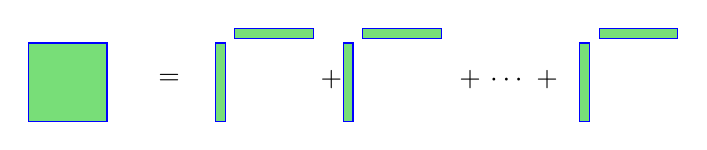
\begin{tikzpicture}[scale=0.25, every node/.style={transform shape}]
	\pgfmathsetmacro{\cubex}{4}
	\pgfmathsetmacro{\cubey}{4}
	\pgfmathsetmacro{\cubez}{4}
	\draw[blue,fill=pastelgreen] (0,0,0) -- ++(-\cubex,0,0) -- ++(0,-\cubey,0) -- ++(\cubex,0,0) -- cycle;
	%%\draw[blue,fill=pastelgreen] (0,0,0) -- ++(0,0,-\cubez) -- ++(0,-\cubey,0) -- ++(0,0,\cubez) -- cycle;
	%%\draw[blue,fill=pastelgreen] (0,0,0) -- ++(-\cubex,0,0) -- ++(0,0,-\cubez) -- ++(\cubex,0,0) -- cycle;
	
	\node[draw=none, text=black, scale=4] at (2,-3,-3) {$=$};
	\pgfmathsetmacro{\smallwidth}{0.5}
	\draw[blue,fill=pastelgreen] (\cubex+2,0,0) -- ++(-\smallwidth,0,0) -- ++(0,-\cubey,0) -- ++(\smallwidth,0,0) -- cycle;
	\draw[blue,fill=pastelgreen] (\cubex+2 +\cubex + 0.5,0.75,0) -- ++(-\cubex,0,0) -- ++(0,-\smallwidth,0) -- ++(\cubex,0,0) -- cycle;
	%%\draw[blue,fill=pastelgreen] (\cubex+2,0.5,0) -- ++(-\smallwidth,0,0) -- ++(0,0,-\cubez) -- ++(\smallwidth,0,0) -- cycle;
	
	\node[draw=none, text=black, scale=4] at (2+\cubex+4.25,-3,-3) {$+$};
	
	\draw[blue,fill=pastelgreen] (\cubex+2.5 + \cubex+2,0,0) -- ++(-\smallwidth,0,0) -- ++(0,-\cubey,0) -- ++(\smallwidth,0,0) -- cycle;
	\draw[blue,fill=pastelgreen] (\cubex+2.5+\cubex+2 +\cubex + 0.5,0.75,0) -- ++(-\cubex,0,0) -- ++(0,-\smallwidth,0) -- ++(\cubex,0,0) -- cycle;
	%%\draw[blue,fill=pastelgreen] (\cubex+2.5+\cubex+2,0.5,0) -- ++(-\smallwidth,0,0) -- ++(0,0,-\cubez) -- ++(\smallwidth,0,0) -- cycle;
	
	\node[draw=none, text=black, scale=4] at (2+\cubex+5 + \cubex+ 4.25, -3,-3) {$+$ $\cdots$ $+$};
	
	\draw[blue,fill=pastelgreen] (12 + \cubex+2.5 + \cubex+2,0,0) -- ++(-\smallwidth,0,0) -- ++(0,-\cubey,0) -- ++(\smallwidth,0,0) -- cycle;
	\draw[blue,fill=pastelgreen] (12+\cubex+2.5+\cubex+2 +\cubex + 0.5,0.75,0) -- ++(-\cubex,0,0) -- ++(0,-\smallwidth,0) -- ++(\cubex,0,0) -- cycle;
	%%\draw[blue,fill=pastelgreen] (12 + \cubex+2.5+\cubex+2,0.5,0) -- ++(-\smallwidth,0,0) -- ++(0,0,-\cubez) -- ++(\smallwidth,0,0) -- cycle;
	\end{tikzpicture}
\end{center}
\end{frame}
\begin{frame}{Popular Tensor Decompositions}{Higher Order Generalization of SVD}
\begin{itemize}
\item Canonical decomposition (equivalently known as Canonical Polyadic or CANDECOMP or PARAFAC)
\vfill
\item Tucker decomposition
\vfill
\item Tensor Train decomposition (equivalently known as Matrix Product States)
\vfill
\end{itemize}
\begin{block}{Tensor Notations}
\begin{itemize}
	\item \tensor{A} $\in \mathbb{R}^{n_1 \times \ldots \times n_d}$ is a $d$-dimensional tensor
	\item $\tensor{A}(i_1,\cdots,i_d)$ represent elements of $\tensor{A}$
	\item Use bold letters to denote tensors
\end{itemize}
\end{block}
\end{frame}

\begin{frame}{Canonical Representation}
\begin{center}
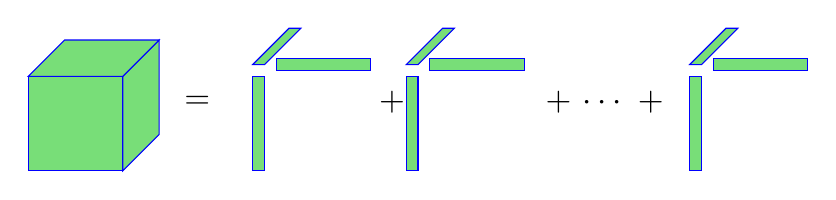
\begin{tikzpicture}[scale=0.3, every node/.style={transform shape}]
\pgfmathsetmacro{\cubex}{4}
\pgfmathsetmacro{\cubey}{4}
\pgfmathsetmacro{\cubez}{4}
\draw[blue,fill=pastelgreen] (0,0,0) -- ++(-\cubex,0,0) -- ++(0,-\cubey,0) -- ++(\cubex,0,0) -- cycle;
\draw[blue,fill=pastelgreen] (0,0,0) -- ++(0,0,-\cubez) -- ++(0,-\cubey,0) -- ++(0,0,\cubez) -- cycle;
\draw[blue,fill=pastelgreen] (0,0,0) -- ++(-\cubex,0,0) -- ++(0,0,-\cubez) -- ++(\cubex,0,0) -- cycle;

\node[draw=none, text=black, scale=4] at (2,-2.25,-3) {$=$};
\pgfmathsetmacro{\smallwidth}{0.5}
\draw[blue,fill=pastelgreen] (\cubex+2,0,0) -- ++(-\smallwidth,0,0) -- ++(0,-\cubey,0) -- ++(\smallwidth,0,0) -- cycle;
\draw[blue,fill=pastelgreen] (\cubex+2 +\cubex + 0.5,0.75,0) -- ++(-\cubex,0,0) -- ++(0,-\smallwidth,0) -- ++(\cubex,0,0) -- cycle;
\draw[blue,fill=pastelgreen] (\cubex+2,0.5,0) -- ++(-\smallwidth,0,0) -- ++(0,0,-\cubez) -- ++(\smallwidth,0,0) -- cycle;

\node[draw=none, text=black, scale=4] at (2+\cubex+4.25,-2.25,-3) {$+$};

\draw[blue,fill=pastelgreen] (\cubex+2.5 + \cubex+2,0,0) -- ++(-\smallwidth,0,0) -- ++(0,-\cubey,0) -- ++(\smallwidth,0,0) -- cycle;
\draw[blue,fill=pastelgreen] (\cubex+2.5+\cubex+2 +\cubex + 0.5,0.75,0) -- ++(-\cubex,0,0) -- ++(0,-\smallwidth,0) -- ++(\cubex,0,0) -- cycle;
\draw[blue,fill=pastelgreen] (\cubex+2.5+\cubex+2,0.5,0) -- ++(-\smallwidth,0,0) -- ++(0,0,-\cubez) -- ++(\smallwidth,0,0) -- cycle;

\node[draw=none, text=black, scale=4] at (2+\cubex+5 + \cubex+ 4.25, -2.25,-3) {$+$ $\cdots$ $+$};

\draw[blue,fill=pastelgreen] (12 + \cubex+2.5 + \cubex+2,0,0) -- ++(-\smallwidth,0,0) -- ++(0,-\cubey,0) -- ++(\smallwidth,0,0) -- cycle;
\draw[blue,fill=pastelgreen] (12+\cubex+2.5+\cubex+2 +\cubex + 0.5,0.75,0) -- ++(-\cubex,0,0) -- ++(0,-\smallwidth,0) -- ++(\cubex,0,0) -- cycle;
\draw[blue,fill=pastelgreen] (12 + \cubex+2.5+\cubex+2,0.5,0) -- ++(-\smallwidth,0,0) -- ++(0,0,-\cubez) -- ++(\smallwidth,0,0) -- cycle;

\end{tikzpicture}
\end{center}

\begin{itemize}
\item $\tensor{A}(i_1,\cdots,i_d) = \sum_{\alpha=1}^{r} U_1(i_1,\alpha) U_2(i_2,\alpha)\cdots U_d(i_d,\alpha)$
%%	\item The minimum value of $r$ is called the canonical rank
\end{itemize}
\medspace
\begin{itemize}
\item ({\color{green}+})  For $n_1=n_2=\cdots n_d=n$, the number of entries = $\mathcal{O}(nrd)$
\item ({\color{red}-}) Determining the minimum value of $r$ is an NP-complete problem
\item ({\color{red}-}) No robust algorithms to compute this representation
\end{itemize}
\end{frame}

\begin{frame}{Tucker Representation}
\begin{center}
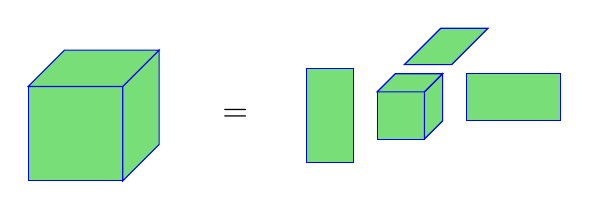
\begin{tikzpicture}[scale=0.3, every node/.style={transform shape}]
\pgfmathsetmacro{\cubex}{4}
\pgfmathsetmacro{\cubey}{4}
\pgfmathsetmacro{\cubez}{4}
\draw[blue,fill=pastelgreen] (-12,1,\cubez-2) -- ++(-\cubex,0,0) -- ++(0,-\cubey,0) -- ++(\cubex,0,0) -- cycle;
\draw[blue,fill=pastelgreen] (-12,1,\cubez-2) -- ++(0,0,-\cubez) -- ++(0,-\cubey,0) -- ++(0,0,\cubez) -- cycle;
\draw[blue,fill=pastelgreen] (-12,1,\cubez-2) -- ++(-\cubex,0,0) -- ++(0,0,-\cubez) -- ++(\cubex,0,0) -- cycle;
\node[draw=none, text=black, scale=4] at (-8,-1,0) {$=$};

\pgfmathsetmacro{\cubex}{2}
\pgfmathsetmacro{\cubey}{2}
\pgfmathsetmacro{\cubez}{2}
\draw[blue,fill=pastelgreen] (0,0,0) -- ++(-\cubex,0,0) -- ++(0,-\cubey,0) -- ++(\cubex,0,0) -- cycle;
\draw[blue,fill=pastelgreen] (0,0,0) -- ++(0,0,-\cubez) -- ++(0,-\cubey,0) -- ++(0,0,\cubez) -- cycle;
\draw[blue,fill=pastelgreen] (0,0,0) -- ++(-\cubex,0,0) -- ++(0,0,-\cubez) -- ++(\cubex,0,0) -- cycle;

\draw[blue,fill=pastelgreen] (-\cubex-1,1,0) -- ++(-\cubex,0,0) -- ++(0,-\cubey-2,0) -- ++(\cubex,0,0) -- cycle;
\draw[blue,fill=pastelgreen] (\cubex+2+1,0,-\cubey) -- ++(-\cubex-2,0,0) -- ++(0,-\cubey,0) -- ++(\cubex+2,0,0) -- cycle;

\draw[blue,fill=pastelgreen] (0,0,-\cubez-1) -- ++(-\cubex,0,0) -- ++(0,0,-\cubez-2) -- ++(\cubex,0,0) -- cycle;
\end{tikzpicture}
\end{center}

\begin{itemize}
\item Represents a tensor with $d$ matrices and a small core tensor
\item $\tensor{A}(i_1,\cdots,i_d) = \sum_{\alpha_1=1}^{r_1}\cdots\sum_{\alpha_d=1}^{r_d} \tensor{g}_{\alpha_1\cdots\alpha_d}U_1(i_1,\alpha_1)$ $\cdots U_d(i_d, \alpha_d)$
\medspace
\end{itemize}
\medspace
\begin{itemize}
\item ({\color{green}+}) SVD based stable algorithms to compute this representation
\item ({\color{red}-})  For $n_1=n_2=\cdots n_d=n$ and $r_1=r_2=\cdots =r_d=r$, the number of entries = $\mathcal{O}(ndr+r^d)$
\end{itemize}	
\end{frame}

%------------------------------------------------
\begin{frame}{Tensor Train Representation: Product of Matrices View}
\begin{itemize}
\item A $d$-dimensional tensor is represented with $2$ matrices and $d$-$2$ $3$-dimensional tensors.
\end{itemize}
\begin{figure}
\begin{center}	
\includegraphics[scale=0.35]{./diagrams/ttentry.eps}
\end{center}
\end{figure}
\noindent An entry of $\tensor{A}$ $\in$ $\mathbb{R}^{n_1 \times \cdots \times n_d}$ is computed by multiplying corresponding matrix (or row/column) of each core.
\end{frame}

\begin{frame}{Tensor Train Representation}

\begin{block}{}
$\tensor{A}$ $\in$ $\mathbb{R}^{n_1 \times \cdots \times n_d}$ is represented with cores $\tensor{G}_k$$\in$ $\mathbb{R}^{r_{k-1}\times n_k\times r_k}$, $k$=$1,2,\cdots d$, $r_0$=$r_d$=$1$ and its elements satisfy the following expression:
{\small\begin{align*}
\tensor{A}(i_1,\cdots ,i_d) 
&= \sum_{\alpha_0 = 1}^{r_0} \cdots \sum_{\alpha_d = 1}^{r_d} \tensor{G}_1(\alpha_0, i_1, \alpha_1) \cdots \tensor{G}_d(\alpha_{d-1}, i_d, \alpha_d)\\
&= \sum_{\alpha_1 = 1}^{r_1} \cdots \sum_{\alpha_{d-1} = 1}^{r_{d-1}} \tensor{G}_1(1, i_1, \alpha_1) \cdots \tensor{G}_d(\alpha_{d-1}, i_d, 1)
\end{align*}}
\begin{center}
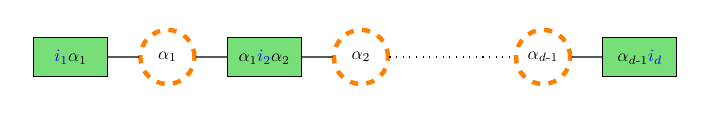
\begin{tikzpicture}[scale=0.625, every node/.style={transform shape}]
\tikzstyle{taskc}=[circle, draw=orange, minimum size=11mm, fill=none, dashed, ultra thick]
\tikzstyle{taskr}=[draw=black, minimum height=8mm, minimum width=15mm, anchor=south west, fill=pastelgreen, text=black]

\node(t1) at (0,0) {};
\node [above right=0cm and 0cm of t1.mid,taskr](T1) {$\textcolor{blue}{i_1}\alpha_1$};
\node [above right=0cm and 0.8cm of T1.south east, taskc](C1) {$\alpha_1$};
\node [above right=0cm and 0.8cm of C1.south east, taskr](T2) {$\alpha_1\textcolor{blue}{i_2}\alpha_2$};
\node [above right=0cm and 0.8cm of T2.south east, taskc](C2) {$\alpha_2$};

\node [above right=0cm and 4.5cm of T2.south east, taskc](Cd) {$\alpha_{d\text{-}1}$};
\node [above right=0cm and 0.8cm of Cd.south east, taskr](Td) {$\alpha_{d\text{-}1}\textcolor{blue}{i_d}$};
\draw (T1.east)--(C1.west);
\draw (C1.east)--(T2.west);
\draw (T2.east)--(C2.west);
\draw [dotted] (C2.east)--(Cd.west);
\draw (Cd.east)--(Td.west);
\path (-0.1, -0.4) -- (2.5, -0.4); 
%%\path (-0.1, -0.8) -- (2.5, -0.8); 
\end{tikzpicture}
\end{center}
\end{block}
\begin{itemize}
\item For $n_1=n_2=\cdots=n_d=n$ and $r_1=r_2=\cdots=r_{d-1}=r$, the number of entries = $\mathcal{O}(ndr^2)$
\end{itemize}
\end{frame}



\begin{frame}
\frametitle{Table of Contents}
\tableofcontents[currentsection]
\end{frame}

%%\subsection{Tensor Train Decomposition}
%%\begin{frame}{Tensor Train Decomposition}
%%content...
%%\end{frame}
%%\begin{frame}{Parallel Tensor Train Decomposition and Approximation Algorithms}
%%content...
%%\end{frame}
\begin{frame}{Unfolding Matrices of a Tensor \& Notations}
\begin{itemize}
	\item Frobenius norm of a matrix $A$ is defined as, $||A||_F = \sqrt{\sum_{i,j} A(i;j)^2}$
	\item Frobenius norm of a $d$-dimensional tensor \tensor{A} is defined as, $||\tensor{A}||_F=$ $\sqrt{\sum_{i_1, i_2, \cdots, i_d}\tensor{A}(i_1,i_2,\cdots, i_d)^2 }$
\end{itemize}
\begin{block}{$k$-th unfolding matrix}
	$A_k$ denotes $k$-th unfolding matrix of tensor $\tensor{A}$ $\in$ $\mathbb{R}^{n_1 \times \cdots \times n_d}$.
	
	$\qquad\qquad A_k = [A_k(i_1, i_2,\cdots, i_k; i_{k+1},\cdots ,i_d)]$
	
	\begin{itemize}
		\item Size of $A_k$ is $(\prod_{l=1}^{k}n_l)\times(\prod_{l=k+1}^{d}n_l)$
		\item $r_k$ denotes the rank of $A_k$.
	\end{itemize}
\end{block}
\begin{itemize}
	\item ($r_1, r_2,\cdots, r_{d-1}$) denotes the ranks of unfolding matrices of the tensor.
\end{itemize}
\end{frame}


\begin{frame}{Separatation of Dimensions \only<1>{in Sequential Algorithms}\only<2>{for Maximum Parallelization}}
\begin{block}{}
	\onslide<1->{
		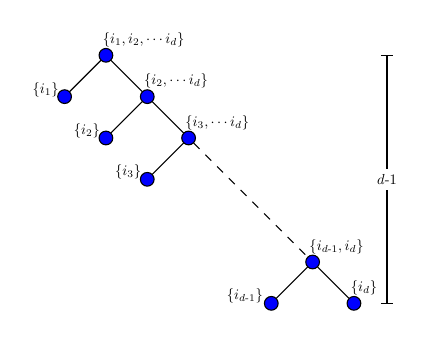
\begin{tikzpicture}[scale=0.525, every node/.style={transform shape}]
		%%\draw[fill=cyan] (0,0) circle (0.8cm);
		%%		\node [draw,circle]{r};
		%%		\tikzstyle{task}=[circle, draw, minimum size=10mm]
		%%		\node (d) at (0,0)[task, fill=babyblueeyes] {$D$};
		%%		\node (e) at (2.5,0)[task, fill=pastelviolet] {$E$};
		%%		\draw[thick, ->] (d.east) -- (e);
		%%		
		%%		\node (a) at (0,2)[task, fill=pastelyellow] {$A$};
		%%		\node (b) at (2.5,2.75)[task, fill=pastelgreen] {$B$};
		%%		\node (c) at (2.5,1.25)[task, fill=pastelred] {$C$};
		%%		
		%%		\draw[thick, ->] (a.east) -- (b);
		%%		\draw[thick, ->] (a.east) -- (c);
		\tikzstyle{taskc}=[circle, draw=black, minimum size=2mm, fill=blue]
		\tikzstyle{taskr}=[draw=none, minimum height=2mm, minimum width=5mm, anchor=south west, fill=none, text=black]
		%%
		\node (t01) at (0,0) [taskc]{};
		\node (t11) at (-1,-1) [taskc] {};
		\node (t12) at (1, -1) [taskc] {};
		\node (t21) at (0, -2) [taskc] {};
		\node (t22) at (2, -2) [taskc] {};
		\node (t31) at (1,-3) [taskc] {};
		\node (t52) at (5, -5) [taskc] {};
		\node (t61) at (4, -6) [taskc] {};
		\node (t62) at (6, -6) [taskc] {};
		
		\draw (t01) -- (t11);
		\draw (t01) -- (t12);
		\draw (t12) -- (t21);
		\draw (t12) -- (t22);
		\draw (t22) -- (t31);
		\draw [dashed] (t22) -- (t52);
		\draw (t52) -- (t61);
		\draw (t52) -- (t62);
		
		\draw (6.8, -6) -- (6.8, -3.25);
		\draw (6.8, -2.75) -- (6.8, 0);
		
		\draw (6.65, -6) -- (6.95, -6);
		\draw (6.65, -0) -- (6.95, 0);
		\node at (6.8, -3) {$d\text{-}1$};
		
		\node [above left=0mm and 2mm of t01.mid, taskr](l01) {$\{i_1,i_2,\cdots i_d\}$};
		\node [below left=2mm and 9mm of t11.mid, taskr](l11) {$\{i_1\}$};
		\node [above left=0mm and 2mm of t12.mid, taskr](l12) {$\{i_2,\cdots i_d\}$};
		\node [below left=2mm and 9mm of t21.mid, taskr](l21) {$\{i_2\}$};
		\node [above left=0mm and 2mm of t22.mid, taskr](l22) {$\{i_3,\cdots i_d\}$};
		\node [below left=2mm and 9mm of t31.mid, taskr](l31) {$\{i_3\}$};
		
		\node [above left=0mm and 2mm of t52.mid, taskr](l52) {$\{i_{d\text{-}1}, i_d\}$};
		\node [below left=2mm and 12mm of t61.mid, taskr](l61) {$\{i_{d\text{-}1}\}$};
		\node [above left=0mm and 2mm of t62.mid, taskr](l62) {$\{i_d\}$};
		
		\path (-0.1, -6.4) -- (2.5, -6.4); 
		\end{tikzpicture}
	}
	\onslide<2->{
		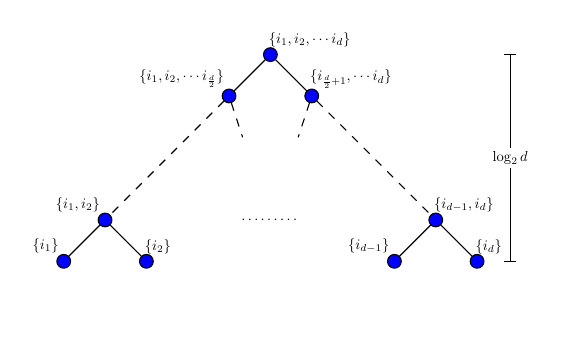
\begin{tikzpicture}[scale=0.525, every node/.style={transform shape}]
		
		\tikzstyle{taskc}=[circle, draw=black, minimum size=2mm, fill=blue]
		%%	\tikzstyle{taskr}=[draw=none, minimum height=2mm, minimum width=5mm, anchor=south west, fill=none, text=black]
		
		
		\node (t01) at (0,0) [taskc]{};
		\node (t11) at (-1,-1) [taskc] {};
		\node (t12) at (1, -1) [taskc] {};
		
		\node (tinter1) at (-0.5,-2) [taskc, draw=none, fill=none] {};
		\node (tinter2) at (0.5,-2) [taskc, draw=none, fill=none] {};
		
		\node (t41) at (-4,-4) [taskc] {};
		\node (t42) at (4,-4) [taskc] {};
		\node (t51) at (-5,-5) [taskc] {};
		\node (t52) at (-3,-5) [taskc] {};
		\node (t53) at (3,-5) [taskc] {};
		\node (t54) at (5,-5) [taskc] {};
		
		
		\draw (t01) -- (t11);
		\draw (t01) -- (t12);
		
		\draw [dashed] (t11) -- (tinter1.west);
		\draw [dashed] (t12) -- (tinter2.east);
		
		\draw [dashed] (t11) -- (t41);
		\draw [dashed] (t12) -- (t42);
		
		\path (t41) -- (t42) node [midway] {$\cdots\cdots\cdots$};
		
		\draw (t41) -- (t51);
		\draw (t41) -- (t52);
		
		\draw (t42) -- (t53);
		\draw (t42) -- (t54);
		
		
		\draw (5.8, -5) -- (5.8, -2.75);
		\draw (5.8, -2.25) -- (5.8, 0);
		
		\draw (5.65, -5) -- (5.95, -5);
		\draw (5.65, 0) -- (5.95, 0);
		\node at (5.8, -2.5) {$\log_2 d$};
		
		\node [above right] at (t01.160) {$\{i_1,i_2,\cdots i_d\}$};	
		
		\node [above left] at (t11.mid) {$\{i_1,i_2,\cdots i_\frac{d}{2}\}$};	
		\node [above right] at (t12.160) {$\{i_{\frac{d}{2}+1},\cdots i_d\}$};
		
		\node [above left] at (t41.mid) {$\{i_1,i_2\}$};
		\node [above right] at (t42.160) {$\{i_{d-1}, i_d\}$};
		
		\node [above left] at (t51.mid) {$\{i_1\}$};
		\node [above right] at (t52.160) {$\{i_2\}$};
		
		\node [above left] at (t53.mid) {$\{i_{d-1}\}$};
		\node [above right] at (t54.160) {$\{i_d\}$};
		
		
		\path (-0.1, -6.4) -- (2.5, -6.4); 
		%%		\path (-6.5, 0) -- (0,0);
		\end{tikzpicture}
	}
\end{block}
\end{frame}


\begin{frame}{Diagramatic Representation of the Algorithm}
\begin{center}
	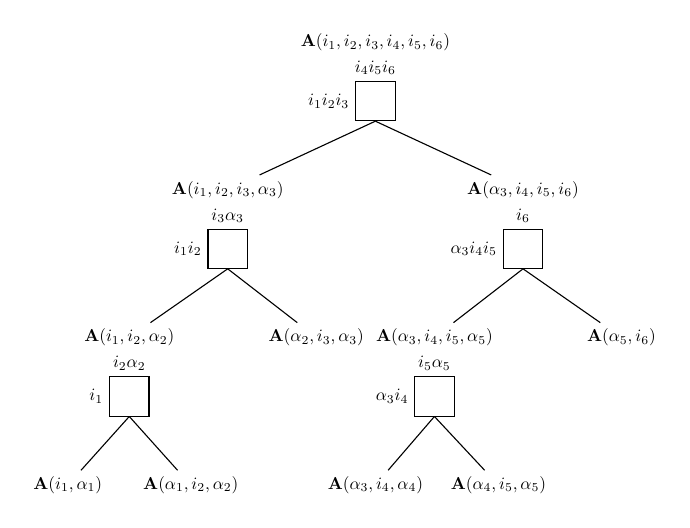
\begin{tikzpicture}[scale=0.625, every node/.style={transform shape}]
	\tikzstyle{taskr}=[draw=black, minimum height=8mm, minimum width=8mm, fill=none, text=black]
	%%	anchor=south west,
	\node (t10) at (0,1.2) {$\tensor{A}(i_1,i_2,i_3,i_4,i_5,i_6)$};	
	\node (b01) at (0,0) [taskr]{};
	\node [above] at (b01.north) {$i_4i_5i_6$};
	\node [left] at (b01.west) {$i_1i_2i_3$};		
	
	\node (t11) at (-3,-1.8) {$\tensor{A}(i_1,i_2,i_3,\alpha_3)$};
	\node (t12) at (3,-1.8) {$\tensor{A}(\alpha_3, i_4, i_5, i_6)$};
	
	\draw (b01.south) -- (t11);	
	\draw (b01.south) -- (t12);
	
	\node (b11) at (-3,-3) [taskr]{};
	\node (b12) at (3,-3) [taskr]{};
	
	\node [above] at (b11.north) {$i_3\alpha_3$};
	\node [left] at (b11.west) {$i_1i_2$};
	
	\node [above] at (b12.north) {$i_6$};
	\node [left] at (b12.west) {$\alpha_3i_4i_5$};
	
	\node (t21) at (-5, -4.8) {$\tensor{A}(i_1,i_2,\alpha_2)$};
	\node (t22) at (-1.2, -4.8) {$\tensor{A}(\alpha_2, i_3,\alpha_3)$};
	
	\node (t23) at (1.2, -4.8) {$\tensor{A}(\alpha_3,i_4,i_5,\alpha_5)$};
	\node (t24) at (5, -4.8) {$\tensor{A}(\alpha_5, i_6)$};
	
	\draw (b11.south) -- (t21);
	\draw (b11.south) -- (t22);
	
	\draw (b12.south) -- (t23);
	\draw (b12.south) -- (t24);		
	
	\node (b21) at (-5,-6) [taskr]{};
	\node [above] at (b21.north) {$i_2\alpha_2$};
	\node [left] at (b21.west) {$i_1$};
	
	\node (b22) at (1.2,-6) [taskr]{};
	\node [above] at (b22.north) {$i_5\alpha_5$};
	\node [left] at (b22.west) {$\alpha_3i_4$};
	
	\node (t31) at (-6.25, -7.8) {$\tensor{A}(i_1,\alpha_1)$};
	\node (t32) at (-3.75, -7.8) {$\tensor{A}(\alpha_1,i_2,\alpha_2)$};
	
	\draw (b21.south) -- (t31);
	\draw (b21.south) -- (t32);
	
	\node (t33) at (0, -7.8) {$\tensor{A}(\alpha_3,i_4,\alpha_4)$};
	\node (t34) at (2.5, -7.8) {$\tensor{A}(\alpha_4,i_5,\alpha_5)$};
	
	\draw (b22.south) -- (t33);
	\draw (b22.south) -- (t34);
	
	\end{tikzpicture}
\end{center}

\begin{theorem}{\small
		If for each unfolding $A_k$ of a $d$-dimensional tensor \tensor{A}, $rank(A_k)=r_k$, then our parallel algorithm produces a Tensor Train representation with ranks not higher than $r_k$.}
\end{theorem}
\end{frame}

\begin{frame}{Sequential Tensor Train Approximation}
\begin{itemize}
	\item Uniform truncation of $\Delta$=$\frac{\epsilon}{\sqrt{d-1}}$ is applied at each step
	\item $\Sigma_2$ is selected based on $\Delta$
	\item Approximation error of this approach is bounded by $\epsilon$
\end{itemize}
\end{frame}

\begin{frame}{Parallel Tensor Train Approximation Algorithms}
\begin{itemize}
	\item We choose $X$, $S$, and $Y$ such that $XSY=\Sigma_1$
	\item We assume $\frac{\epsilon_1^2}{d_1^2} = \frac{\epsilon_2^2}{d_2^2}$
	\item $\Sigma_2$ is selected based on $\Delta$=$ \frac{\epsilon}{\sqrt{d-1}}$
	\item $\epsilon_1$ = f($\epsilon, \epsilon_2, \Delta, X, S, Y$) 
\end{itemize}
 \includegraphics[scale=0.02]{./tmp/leadingSingularValuesPassed-1.jpg}
 \includegraphics[scale=0.02]{./tmp/leadingSingularValuesPassed-2.jpg}
\end{frame}

\begin{frame}{Accuracy of parallel approximation algorithms}
\begin{itemize}
	\item \textit{Leading Singular values to Right subtensor} (\hfirst)
	\item \textit{Square root of Leading Singular values to Both subtensors} (\hsecond)
	\item \textit{Leading Singular values to Both subtensors} (\hthird) 
\end{itemize}
	
\end{frame}

\begin{frame}{Low Rank Functions}
\begin{center}
	\begin{tabular}{|l|c|}
		\hline
		$Log$ & $\log(\sum_{j=1}^{N}j i_j)$\\ \hline
		$Sin$ & $\sin(\sum_{j=1}^{N}i_j)$\\ \hline
		Inverse-Square-Root ($ISR$) & $\frac{1}{\sqrt{\sum_{j=1}^{N}i_j^2}}$\\ \hline
		Inverse-Cube-Root ($ICR$) & $\frac{1}{\sqrt[3]{\sum_{j=1}^{N}i_j^3}}$\\ \hline
		Inverse-Penta-Root ($IPR$) & $\frac{1}{\sqrt[5]{\sum_{j=1}^{N}i_j^5}}$\\ \hline
	\end{tabular}
\end{center}
We consider $N=12$ and $i_j \in \{1, 2, 3, 4\}_{1\le j \le N}$. This setting produces a $12$-dimensional tensor with $4^{12}$ elements for each low rank function. Her we show results only for $Log$ tensor.
\end{frame}

\begin{frame}{Comparison of All Approaches for the $Log$ tensor}
$\color{blue}{\bullet}$ Prescribed accuracy = $10^{-6}$\\
%%$\color{blue}{\bullet}$ Prototyped all approached in Matlab\\
$\color{blue}{\bullet}$ compr: compression ratio, ne: number of elements in aprroximation, OA: approximation accuracy
%%\begin{center}{\small
%%		\begin{tabular}{|c|c|c|c|c|c|c|}
%%			%%		\toprule
%%			\hline
%%			Appr. & Metric & $Log$ & $Sin$ & $ISR$ & $ICR$ & $IPR$\\ \hline
%%			\multirow{3}{*} {\otta} & compr & 99.993 & 99.999 & 99.987 & 99.981 & 99.971 \\ \cline{2-7} 
%%			& ne    & 1212 & 176 & 2240 & 3184 & 4864 \\ \cline{2-7} 
%%			& OA    & 2.271e-07 & 2.615e-09 & 1.834e-07 & 4.884e-07 & 4.836e-07 \\ \cline{1-7} 
%%			\multirow{3}{*} {\hfirst} & compr & 99.817 & 99.998 & 99.915 & 99.874 & 99.824 \\ \cline{2-7} 
%%			& ne    & 30632 & 344 & 14196 & 21176 & 29524 \\ \cline{2-7} 
%%			& OA    & 3.629e-08 & 1.412e-11 & 1.118e-07 & 8.520e-08 & 5.811e-08 \\ \cline{1-7} 
%%			\multirow{3}{*} {\hsecond} & compr & 99.799 & 99.999 & 99.952 & 99.912 & 99.870 \\ \cline{2-7} 
%%			& ne    & 33772 & 176 & 8068 & 14824 & 21792 \\ \cline{2-7} 
%%			& OA    & 2.820e-08 & 6.144e-12 & 1.118e-07 & 8.518e-08 & 5.664e-08 \\ \cline{1-7} 
%%			\multirow{3}{*} {\hthird} & compr & 99.993 & 99.999 & 99.987 & 99.981 & 99.970 \\ \cline{2-7} 
%%			& ne    & 1212 & 176 & 2240 & 3184 & 4964 \\ \cline{2-7} 
%%			& OA    & 2.265e-07 & 1.252e-11 & 1.834e-07 & 4.884e-07 & 3.999e-07 \\ \cline{1-7} 
%%		\end{tabular}
%%}\end{center}

\begin{center}
	\begin{tabular}{|c|c|c|c|}
		\hline
		Approach & compr & ne & OA\\ \hline
		\otta & 99.993 & 1212 & 2.271e-07 \\ \hline
		\hfirst & 99.817 & 30632 & 3.629e-08 \\ \hline
		\hsecond & 99.799 & 33772 & 2.820e-08 \\ \hline
		\hthird & 99.993 & 1212 & 2.265e-07 \\ \hline
	\end{tabular}
\end{center}
\end{frame}

\begin{frame}{Accuracy Results}
\begin{itemize}
	\item SVD is expensive -- we also experimented with QRCP and Randomized SVD
\end{itemize}
\begin{center}
	\begin{tabular}{|c|c|c|c|c|}
		\hline
		Approach & Rank & compr & ne & OA\\ \hline
		SVD & 5 & 99.994 & 992 & 6.079e-06\\ \hline
		QRCP & 5 & 99.994 & 992 & 1.016e-05\\ \hline
		RSVD & 5 & 99.994 & 992 & 6.0791e-06\\ \hline
		
		SVD & 6 & 99.992 & 1376 & 1.323e-07\\ \hline
		QRCP & 6 & 99.992 & 1376 & 3.555e-07\\ \hline
		RSVD & 6 & 99.992 & 1376 & 1.3228e-07\\ \hline
		
		SVD & 7 & 99.989 & 1824 & 2.753e-09\\ \hline
		QRCP & 7 & 99.989 & 1824 & 6.620e-09\\ \hline
		RSVD & 7 & 99.989 & 1824 & 2.7602e-09\\ \hline
%%		
%%		\otta & 99.993 & 1212 & 2.271e-07 \\ \hline
%%		\hfirst & 99.817 & 30632 & 3.629e-08 \\ \hline
%%		\hsecond & 99.799 & 33772 & 2.820e-08 \\ \hline
%%		\hthird & 99.993 & 1212 & 2.265e-07 \\ \hline
	\end{tabular}
\end{center}
\end{frame}


\begin{frame}{Performance Comparison}
\begin{itemize}
	\item Computation cost of the parallel algorithm decreases exponentially at each step
	\item Each algorithm runs on $P$ processors
\end{itemize}
Cost along the critical path:
\begin{center}
	\begin{tabular}{|c|c|c|c|}
		\hline
		Algorithm & Computation cost & Communication volume & Number of Messages\\ \hline
		Sequential & $\mathcal{O}(\frac{N^d}{P})$ & $\mathcal{O}(\frac{N^d}{\sqrt{P}}\log{}P)$ & $\mathcal{O}(d\log{}P)$\\ \hline
		Parallel & $\mathcal{O}(\frac{N^d}{P})$ & $\mathcal{O}(\frac{N^d}{\sqrt{P}}\log{}P)$ & $\mathcal{O}(\log{}d \log{}P)$\\ \hline
%%		$\mathcal{O}(n\log{}n)$ 
	\end{tabular}
\end{center}

Cost along the critical path after the first step,
\begin{center}
	\begin{tabular}{|c|c|c|c|}
		\hline
		Algorithm & Computation cost & Communication volume & Number of Messages\\ \hline
		Sequential & $\mathcal{O}(\frac{N^{d-1}}{P})$ & $\mathcal{O}(\frac{N^{d-1}}{\sqrt{P}}\log{}P)$ & $\mathcal{O}(d\log{}P)$\\ \hline
		Parallel & $\mathcal{O}(\frac{N^\frac{d}{2}}{P})$ & $\mathcal{O}(\frac{N^\frac{d}{2}}{\sqrt{P}}\log{}P)$ & $\mathcal{O}(\log{}d \log{}P)$\\ \hline
		%%		$\mathcal{O}(n\log{}n)$ 
	\end{tabular}
\end{center}
\end{frame}



\subsection{Communication Optimal Algorithms for Tensors}


\begin{frame}
\frametitle{Table of Contents}
\tableofcontents[currentsubsection]
\end{frame}

\begin{frame}{Why Communication is Important?}
\begin{itemize}
	\item Running time of an algorithm depends on 
	\begin{itemize}
		\item Number of computations * time-per-computation
		\item Data movement
		\begin{itemize}
			\item Volume of communication / Network-bandwidth
			\item Number of messages * Network-latency
		\end{itemize}
	\end{itemize}
	\item Gaps growing exponentially with time (Source: Getting up to speed: The future of supercomputing)
	
%%	\begin{center}
	\begin{tabular}{|c|c|}
		\hline
		\multicolumn{2}{|c|}{Annual improvements}\\ \hline
		time-per-computation & 59\%\\ \hline
		Network-bandwidth & 26\%\\ \hline
		Network-latency & 15 \% \\ \hline
	\end{tabular}
%%	\end{center}
%%\credit{Getting up to speed: The future of supercomputing}
\item Avoid communication to save time (and energy)
\end{itemize}

\includegraphics[scale=0.02]{./tmp/networkTopology.jpg}
%%Source: GETTING UP TO SPEED THE FUTURE OF SUPERCOMPUTING
%%Figures fromGetting up to speed:  The future of supercomputing, 2005,National Academies Press (2004 figure based on data on the period 1988-2002)
\end{frame}

\begin{frame}{Communication Optimal Algorithms for Tensors}
	 \begin{columns}
	\begin{column}[c]{.25\textwidth}
%%		\includegraphics[width=\textwidth]{figs/sunway-taihulight.jpg}
	\end{column}
	\begin{column}[c]{.75\textwidth}
		\includegraphics[scale=0.25]{./diagrams/ttentry}
	\end{column}
\end{columns}
\begin{itemize}
	\item This is a hard problem to start with
	\item We look similar computation which has simpler structure than this
\end{itemize}
\begin{block}{3-dimensional Multiple Tensor Times Matrix (Multi TTM)}
	\begin{center}
		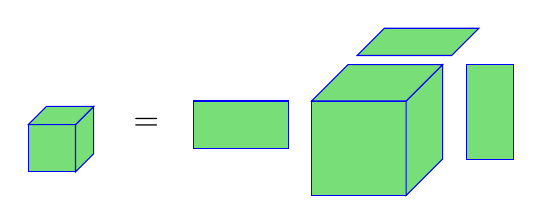
\begin{tikzpicture}[scale=0.3, every node/.style={transform shape}]
		\pgfmathsetmacro{\cubex}{2}
		\pgfmathsetmacro{\cubey}{2}
		\pgfmathsetmacro{\cubez}{2}
		\draw[blue,fill=pastelgreen] (-14,-1,\cubez-2) -- ++(-\cubex,0,0) -- ++(0,-\cubey,0) -- ++(\cubex,0,0) -- cycle;
		\draw[blue,fill=pastelgreen] (-14,-1,\cubez-2) -- ++(0,0,-\cubez) -- ++(0,-\cubey,0) -- ++(0,0,\cubez) -- cycle;
		\draw[blue,fill=pastelgreen] (-14,-1,\cubez-2) -- ++(-\cubex,0,0) -- ++(0,0,-\cubez) -- ++(\cubex,0,0) -- cycle;
		\node[draw=none, text=black, scale=4] at (-11,-1,0) {$=$};
		
		\pgfmathsetmacro{\cubex}{4}
		\pgfmathsetmacro{\cubey}{4}
		\pgfmathsetmacro{\cubez}{4}
		
		\pgfmathsetmacro{\xs}{2}
		\pgfmathsetmacro{\ys}{2}
		\pgfmathsetmacro{\zs}{2}
		
		\draw[blue,fill=pastelgreen] (0,0,0) -- ++(-\cubex,0,0) -- ++(0,-\cubey,0) -- ++(\cubex,0,0) -- cycle;
		\draw[blue,fill=pastelgreen] (0,0,0) -- ++(0,0,-\cubez) -- ++(0,-\cubey,0) -- ++(0,0,\cubez) -- cycle;
		\draw[blue,fill=pastelgreen] (0,0,0) -- ++(-\cubex,0,0) -- ++(0,0,-\cubez) -- ++(\cubex,0,0) -- cycle;
		
		\draw[blue,fill=pastelgreen] (-\cubex-1,0,0) -- ++(-\cubex,0,0) -- ++(0,-\ys,0) -- ++(\cubex,0,0) -- cycle;
		
		\draw[blue,fill=pastelgreen] (\xs+1,0,-\cubey) -- ++(-\xs,0,0) -- ++(0,-\cubey,0) -- ++(\xs,0,0) -- cycle;
		
		\draw[blue,fill=pastelgreen] (0,0,-\cubez-1) -- ++(-\cubex,0,0) -- ++(0,0,-\zs-1) -- ++(\cubex,0,0) -- cycle;
		\end{tikzpicture}
	\end{center}
\end{block}
\end{frame}


%\begin{frame}
%\end{frame}

\begin{frame}{Revisiting Matrix Multiplication Algorithms}
\begin{itemize}
	\item We look at the existing approaches
	\item Communication lower bounds  fo many computations are mostly derived based on matrix multiplication bounds
	\item Our goal is to express existing approaches in the form suitable for tensors
\end{itemize}

\begin{block}{Communication Optimal Matrix Multiplication Algorithm}
\includegraphics[scale=0.02]{./tmp/3d-mm.jpg}
\end{block}
\begin{itemize}
	\item Reinvented many times: Dekel, Nassimi, Sahni [81], Bernsten [89], Agarwal, Chandra, Snir [90], Johnson [93], Agarwal, Balle, Gustavson, Joshi, Palkar [95]
\end{itemize}
\end{frame}
\begin{frame}{Processors Arranged in Different Ways}
Assume $n_1 \le n_2 \le n_3$ and dimensions of $A$, $B$, and $C$ are $n_2 \times n_1$, $n_1\times n_3$ and $n_2 \times n_3$ respectively.
\begin{block}{Three different arrangements of processor grids}

\includegraphics[scale=0.02]{./tmp/processorRearrangement.jpg}
\end{block}
\end{frame}
\begin{frame}{Lower Bounds for Matrix Multiplication Algorithms}

\includegraphics[scale=0.02]{./tmp/loomisWhitney.jpg}
From Loomis-Whitney inequality,
\begin{align*}
V_x V_y V_z \ge& V^2
\end{align*}
Atleast one processor will perform atleast $\frac{n_1n_2n_3}{P}$ computations. From Loomis-Whitney inequality, $\phi_A \phi_B \phi_C \ge \Big(\frac{n_1n_2n_3}{P}\Big)^2$.

Here $\phi_A$, $\phi_B$ and $\phi_C$ denote the projections of computations on $A$, $B$ and $C$ matrices. Our goal is to minimize $\phi_A + \phi_B + \phi_C$.

We also added other inequalities.
\begin{itemize}
	\item To perform atleast $\frac{1}{P}$th computation, the processor must access atleast $\frac{1}{P}$th data of each matrix
	\item Projectin on each matrix can not be larger than the original matrix
\end{itemize} 
We obtain the following additional inequalities.
\begin{align*}
\frac{n_1n_2}{P} \le \phi_A & \le n_1n_2\\
\frac{n_1n_3}{P} \le \phi_B & \le n_1n_3\\
\frac{n_2n_3}{P} \le \phi_C & \le n_2n_3
\end{align*}

\end{frame}
\begin{frame}{Lower Bounds for Matrix Multiplication Algorithms}
After solving the minimization problem we obtain the following ranges for different arrangement of process grids.

\begin{itemize}
	\item We corrected the constants in the existing ranges of $P$ (Demmel, Eliahu, Fox, Kamil, Lipshitz, Schwartz, Spillinger [IPDPS 2013])
\end{itemize}
\end{frame}
%%\begin{frame}{Multiple Tensor Times Matrix (Multi-TTM) Computations}
%%content...
%%\end{frame}
\begin{frame}{Lower Bounds for Multi-TTM Computations}
\begin{block}{3-dimensional Multiple Tensor Times Matrix (Multi TTM)}
	\begin{center}
		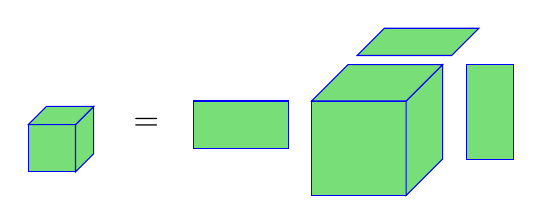
\begin{tikzpicture}[scale=0.3, every node/.style={transform shape}]
		\pgfmathsetmacro{\cubex}{2}
		\pgfmathsetmacro{\cubey}{2}
		\pgfmathsetmacro{\cubez}{2}
		\draw[blue,fill=pastelgreen] (-14,-1,\cubez-2) -- ++(-\cubex,0,0) -- ++(0,-\cubey,0) -- ++(\cubex,0,0) -- cycle;
		\draw[blue,fill=pastelgreen] (-14,-1,\cubez-2) -- ++(0,0,-\cubez) -- ++(0,-\cubey,0) -- ++(0,0,\cubez) -- cycle;
		\draw[blue,fill=pastelgreen] (-14,-1,\cubez-2) -- ++(-\cubex,0,0) -- ++(0,0,-\cubez) -- ++(\cubex,0,0) -- cycle;
		\node[draw=none, text=black, scale=4] at (-11,-1,0) {$=$};
		
		\pgfmathsetmacro{\cubex}{4}
		\pgfmathsetmacro{\cubey}{4}
		\pgfmathsetmacro{\cubez}{4}
		
		\pgfmathsetmacro{\xs}{2}
		\pgfmathsetmacro{\ys}{2}
		\pgfmathsetmacro{\zs}{2}
		
		\draw[blue,fill=pastelgreen] (0,0,0) -- ++(-\cubex,0,0) -- ++(0,-\cubey,0) -- ++(\cubex,0,0) -- cycle;
		\draw[blue,fill=pastelgreen] (0,0,0) -- ++(0,0,-\cubez) -- ++(0,-\cubey,0) -- ++(0,0,\cubez) -- cycle;
		\draw[blue,fill=pastelgreen] (0,0,0) -- ++(-\cubex,0,0) -- ++(0,0,-\cubez) -- ++(\cubex,0,0) -- cycle;
		
		\draw[blue,fill=pastelgreen] (-\cubex-1,0,0) -- ++(-\cubex,0,0) -- ++(0,-\ys,0) -- ++(\cubex,0,0) -- cycle;
		
		\draw[blue,fill=pastelgreen] (\xs+1,0,-\cubey) -- ++(-\xs,0,0) -- ++(0,-\cubey,0) -- ++(\xs,0,0) -- cycle;
		
		\draw[blue,fill=pastelgreen] (0,0,-\cubez-1) -- ++(-\cubex,0,0) -- ++(0,0,-\zs-1) -- ++(\cubex,0,0) -- cycle;
		\end{tikzpicture}
	\end{center}
\end{block}
Let $G$ and $\chi$ are output and input tensors. $A$, $B$ and $C$ are factor matrices, which are multiplied to the input tensor in 1st, 2nd and 3rd dimensions. Sequential code for this computation can be written as..

\end{frame}

\begin{frame}{3-dimensional Multi TTM Computation}
	\begin{algorithmic}
	\FOR{$i_1=1:n_1$}
	\FOR{$i_2=1:n_2$}
	\FOR{$i_3=1:n_3$}
	\FOR{$j_1=1:r_1$}
	\FOR{$j_2=1:r_2$} 
	\FOR{$j_3=1:r_3$} 
	\STATE {$\tensor{G}(j_1,j_2, j_3) += \tensor{X}(i_1,i_2,i_3)*A(i_1,j_1)*B(i_2,j_2)*B(i_3,j_3)$} 
	\ENDFOR 	
	\ENDFOR 	
	\ENDFOR 
	\ENDFOR
	\ENDFOR
	\ENDFOR
\end{algorithmic}
\end{frame}

\begin{frame}{Multi TTM Computation}
$\phi_x$ denotes the projection of iteration space on variable $x$. Here $x\in {G, \mathcal{X}, A, B, C}$. Dimension of $\tensor{G}$, $\mathcal{X}$, $A$, $B$, $C$ are $r_1\times r_2 \times r_3$, $n_1 \times n_2 \times n_3$, $n_1 \times r_1$, $n_2 \times r_2$ and $n_3 \times r_3$ respectively. We assume $r_1r_2r_3 \le n_1n_2n_3$ and $n_1r_1 \le n_2r_2 \le n_3r_3$.

We need to solve the following linear program:

Minimize $\phi_G + \phi_X + \phi_A +\phi_A +\phi_B + \phi_C$ subject to
\begin{align*}
\phi_G \phi_X \ge & \frac{n_1n_2n_3r_1r_2r_3}{P}\\
\phi_A \phi_B \phi_C \ge & \frac{n_1n_2n_3r_1r_2r_3}{P}\\
\frac{n_1n_2n_3}{P} \le \phi_X \le& n_1n_2n_3\\
\frac{r_1r_2r_3}{P} \le \phi_G \le& r_1r_2r_3\\
\frac{n_1r_1}{P} \le \phi_A \le& n_1r_1\\
\frac{n_2r_2}{P} \le \phi_B \le& n_2r_2\\
\frac{n_3r_3}{P} \le \phi_C \le& n_3r_3
\end{align*}

After solving this linear program, we obtain  different communication lower bounds based on the number of processors ($P$) used.
\end{frame}


\begin{frame}{Multi TTM Computation}
\includegraphics[scale=0.02]{./tmp/processorRangeMultiTMM.jpg}
Lower bound on the communication for the processor $\ge $ $\phi_G + \phi_X + \phi_A +\phi_A +\phi_B + \phi_C$ - \textit{Portion of the variables already present in the memory}
\end{frame}


\section{Scheduling on Heterogeneous Resources}
\begin{frame}
\frametitle{Table of Contents}
\tableofcontents[currentsection]
\end{frame}

\subsection{Communication Computation Overlap}
\begin{frame}
\frametitle{Table of Contents}
\tableofcontents[currentsubsection]
\end{frame}

\begin{frame}{Problem Definition}
\begin{columns}
\begin{column}{0.65\textwidth}
\begin{tabular}{|ccc|}
	\hline
	Task & Data Transfer Time & Computation Time\\ \hline
	A & 5 & 3 \\
	B & 2 & 4 \\ \hline
\end{tabular}
\end{column}
\begin{column}{0.35\textwidth}
%%\includegraphics[scale=0.15]{imagefile}
\end{column}
\end{columns}

Problem: Given a set of tasks in what order we transfer them from $M$ to $C$ such that the makespan is minimal?

%%\includegraphics[scale=0.2]{imagefile}

%%\begin{block}{Problem $DT$ }
%%	\begin{itemize}
%%		\item A set of tasks $ST=\{T_1, \cdots, T_n\}$ is scheduled on a processing unit $P$ with
%%		memory unit $M$ of capacity $C$
%%		\item Input data for tasks of $ST$
%%		reside on another memory unit
%%		\item Tasks do not produce output data
%%		\item Tasks do not require intermediate memory
%%		\item A tasks uses an amount of memory in $M$ from the
%%		start of its communication to the end of its computation
%%	\end{itemize}
%%	\noindent Given $L$, is there a feasible schedule $S$ for $ST$ such that
%%	makespan of $S$, $\mu(S) \le L$?
%%\end{block}
\end{frame}

\begin{frame}[fragile]{Order of Data Transfers}
\begin{itemize}
	\item Compute intensive task: Computation time $\ge$ Data transfer time
	\item Communication intensive task: Computation time $<$ Data transfer time
\end{itemize}
\begin{block}{Optimal Algorithm: When memory of the compute unit is not a concern}
	\begin{itemize}
		\item First sort compute intensive tasks in increasing order of their data transfer time
		\item Then sort the communication intensive tasks in decreasing order of their computation time 
	\end{itemize}
\end{block}

\newcommand{\threepart}{\textsc{3Par}\xspace}
\begin{block}{Memory capacity is limited}
	\begin{itemize}
		\item The problem is NP-Complete
		\begin{itemize}
			\item Reduced \threepart problem to this problem
		\end{itemize} 
	   \item Proposed static and dynamic based approaches and evaluated them on traces of molecular simulations 
	\end{itemize}

\tikzset{xtick/.style={inner xsep=0pt, inner ysep=3pt, minimum size=0pt, draw},%
	task/.style args={#1start#2length#3res#4color#5}{rounded corners, draw, inner sep=0pt, fill=#5, label=center:#1, fit={(#2,#4*0.75) (#2+#3,#4*0.75+0.75)}},%
	vert/.style={inner sep=1pt, fill=black, circle, draw, label=#1}
}
\newcommand{\scheduleNoName}[1]{
	\draw[->] (-0.4, 0) -- (#1, 0) node[below] {$t$};
	\draw (0, 0) -- (0, 1.5) node[pos=0.25, left] {Comp.}
	node[pos=0.75, left] {Comm.};
	\draw[dashed,gray] (0, 0.75) -- (#1, 0.75);
}


\begin{center}
	\begin{tikzpicture}[yscale=0.7, thick, xscale=0.6]
	\scheduleNoName{12.5}
	\node[task=$A_{1,1}$ start 0 length 1 res 1 color cyan]{};
	\node[task=$A_{1,2}$ start 1 length 1 res 1 color blue!40!white]{};
	\node[task=$A_{1,3}$ start 2 length 1 res 1 color blue!70!white]{};
	\node[task=$K_0$ start 0 length 3 res 0 color gray!40!white]{};
	\node[task=$K_1$ start 3 length 6 res 1 color green]{}; 
	\node[task=$A_{1,1}$ start 3 length 1.8 res 0 color cyan]{};
	\node[task=$A_{1,2}$ start 4.8 length 2.3 res 0 color blue!40!white]{};
	\node[task=$A_{1,3}$ start 7.1 length 1.9 res 0 color blue!70!white]{};
	\node[task=$A_{2,1}$ start 9 length 1 res 1 color cyan]{};
	\node[task=$A_{2,2}$ start 10 length 1 res 1 color blue!40!white]{};
	\node[task=$A_{2,3}$ start 11 length 1 res 1 color blue!70!white]{};
	\node[task=$K_1$ start 9 length 3 res 0 color green]{};
%%	\draw[<->,thin] (0, -0.2) -- node[below]{$3$} (3, -0.2) ;
%%	\draw[<->,thin] (9, -0.2) -- node[below]{$3$} (12, -0.2) ;
%%	\draw[<->,thin] (3, -0.2) -- node[below]{$b'$} (9, -0.2) ;
	\draw[<->,thin] (0, -0.2) -- (3, -0.2) ;
	\draw[<->,thin] (9, -0.2) -- (12, -0.2) ;
	\draw[<->,thin] (3, -0.2) -- (9, -0.2) ;
	\end{tikzpicture}
\end{center}
\end{block}
\end{frame}


%%\begin{frame}{NP-Completeness Structure}
%%content...
%%\end{frame}
\begin{frame}{Performance evaluation on Summit supercomputer}


\begin{itemize}
	\item TAMM: Tensor Algebra for Manybody Methods
	\item CCSD application, molecule, cc-pVDZ (737 basis functions, 220 nodes), aug-cc-pVDZ (1243 basis functions, 256 nodes)
\end{itemize}
\begin{columns}
	\begin{column}{0.56\linewidth}
		\begin{center}
			\includegraphics[scale=0.13]{./diagrams/Summit_Node.jpg}
			
			\vspace*{-0.25cm}{\tiny \hspace*{2cm} Fig source: \url{https://www.olcf.ornl.gov}}
		\end{center}
	\end{column}
	\begin{column}{0.45\linewidth}
		\includegraphics[scale=0.5]{./diagrams/tamm-performance.eps}
	\end{column}
\end{columns}
\end{frame}



%%\begin{frame}{NWChemEX and TAMM}
%%content...
%%\end{frame}



\subsection{Scheduling of Dense Linear Algebra Kernels}
\begin{frame}
\frametitle{Table of Contents}
\tableofcontents[currentsubsection]
\end{frame}

\begin{frame}{Performance Share of Accelerators: TOP500 list}
\begin{center}
	\begin{tabular}{|c|c|c|}
		\hline
		Year & \#Systems & \% Performance share\\ \hline
		2015 & 103 & 28\\ \hline
		2020 & 147 & 43\\ \hline
	\end{tabular}
\end{center}

%%\begin{block}{}
%%\begin{center}
%%	\begin{tabular}{|c|c|c|}
%%		\hline
%%		Year & \#Systems & \% Performance share\\ \hline
%%		2015 & 103 & 28\\ \hline
%%		2020 & 147 & 43\\ \hline
%%	\end{tabular}
%%\end{center}
%%%%	\begin{itemize}
%%%%		\item {\footnotesize Significant percentage of performance share relies on accelerators}  
%%%%	\end{itemize}
%%\end{block}

\begin{block}{Task Based Runtime Systems}
\begin{itemize}
	%%	\item Challenges:
	%%	\begin{itemize}
	%%%%		\item Scheduling and resource allocation problems are NP hard
	\item Almost impossible to develop optimized hand tune kernels for all architectures
	%%%%		\item Hard to obtain precise estimation of duration of tasks and data transfers
	%%	\end{itemize}
	\vfill
	\item Task based runtime systems
	\begin{itemize}
		\item Eg: StarPU, StarSs, SuperMatrix, QUARK, XKaapi or PaRSEC

		\begin{columns}
			\null \hfill
			\begin{column}{0.35\linewidth}
				\begin{center}
					\includegraphics[scale=0.2]{./diagrams/taskGraph.eps}
				\end{center}
			\end{column}
			\begin{column}{0.65\linewidth}
				\begin{itemize}
					\item Application is represented as a Direct Acyclic Graph (DAG)
					\item Vertices represent tasks
					\item Edges represent dependencies among tasks
				\end{itemize}
			\end{column}
		\end{columns}
		%%		\item Vertices represent tasks and edges represent dependencies among those tasks
		%%		\item Scheduling based on different heuristics
%%		\item Enhance productivity and portability
	\end{itemize}
\end{itemize}
\end{block}
\end{frame}

\begin{frame}{Tiled Cholesky Factorization}	
	%  MAy be here we can mention that we are using Code from Chameleon dense linear algebra library
	\vfill 
	Input: a positive definite matrix, A with N $\times$ N tiles \\
	Output: a lower triangular matrix L, A = LL$^\intercal$
	\begin{algorithm}[H]
		\begin{algorithmic}[1]
			\FOR {$k = 0$ to $N-1$}
			\STATE L[k][k] $\leftarrow$ \textcolor{yellow}{POTRF}(A[k][k])\;
			\FOR {$i = k+1$ to $N-1$}
			\STATE L[i][k] $\leftarrow$ \textcolor{blue}{TRSM}(L[k][k], A[i][k])\;
			\ENDFOR
			\FOR {$j = k+1$ to $N-1$}
			\STATE A[j][j] $\leftarrow$ \textcolor{cyannew}{SYRK}(L[j][k], A[j][j])\;
			\FOR {$i = j+1$ to $N-1$}
			\STATE A[i][j] $\leftarrow$ \textcolor{greenhtml}{GEMM}(L[i][k], L[j][k], A[i][j])\;
			\ENDFOR
			\ENDFOR
			\ENDFOR
			
		\end{algorithmic}
		\caption{Pseudocode of the tiled Cholesky factorization}
	\end{algorithm}
\end{frame}

\begin{frame}{Tiled Cholesky Task Graph (N=5)}	
	\begin{figure}[htb]
		%  \begin{block}{}
		%\centering \includegraphics[scale=0.20]{fig-GP-2016/cholesky_5.pdf}
		\centering 
		%%		\includegraphics[scale=0.20]{fig-GP-2016/readable/cholesky_5.pdf}
		%%		\includegraphics[scale=0.20]{figs/CholeskyTaskGraphs/test1.pdf}
		\includegraphics[scale=0.20]{./diagrams/cholesky_5.pdf}
		%  \end{block}
		
	\end{figure}
	{\footnotesize
		\begin{itemize}
			%%			\item Does not need synchronization at each outer iteration
			\item Exhibits complex dependencies pattern
		\end{itemize}
	}	
\end{frame}


\begin{frame}{Tiled Cholesky Task Graph (N=5)}
	\begin{figure}[htb]
		%  \begin{block}{}
		%\centering \includegraphics[scale=0.20]{fig-GP-2016/cholesky_5.pdf}
		\centering 
		%%		\includegraphics[scale=0.20]{figs/readable/test.pdf}
		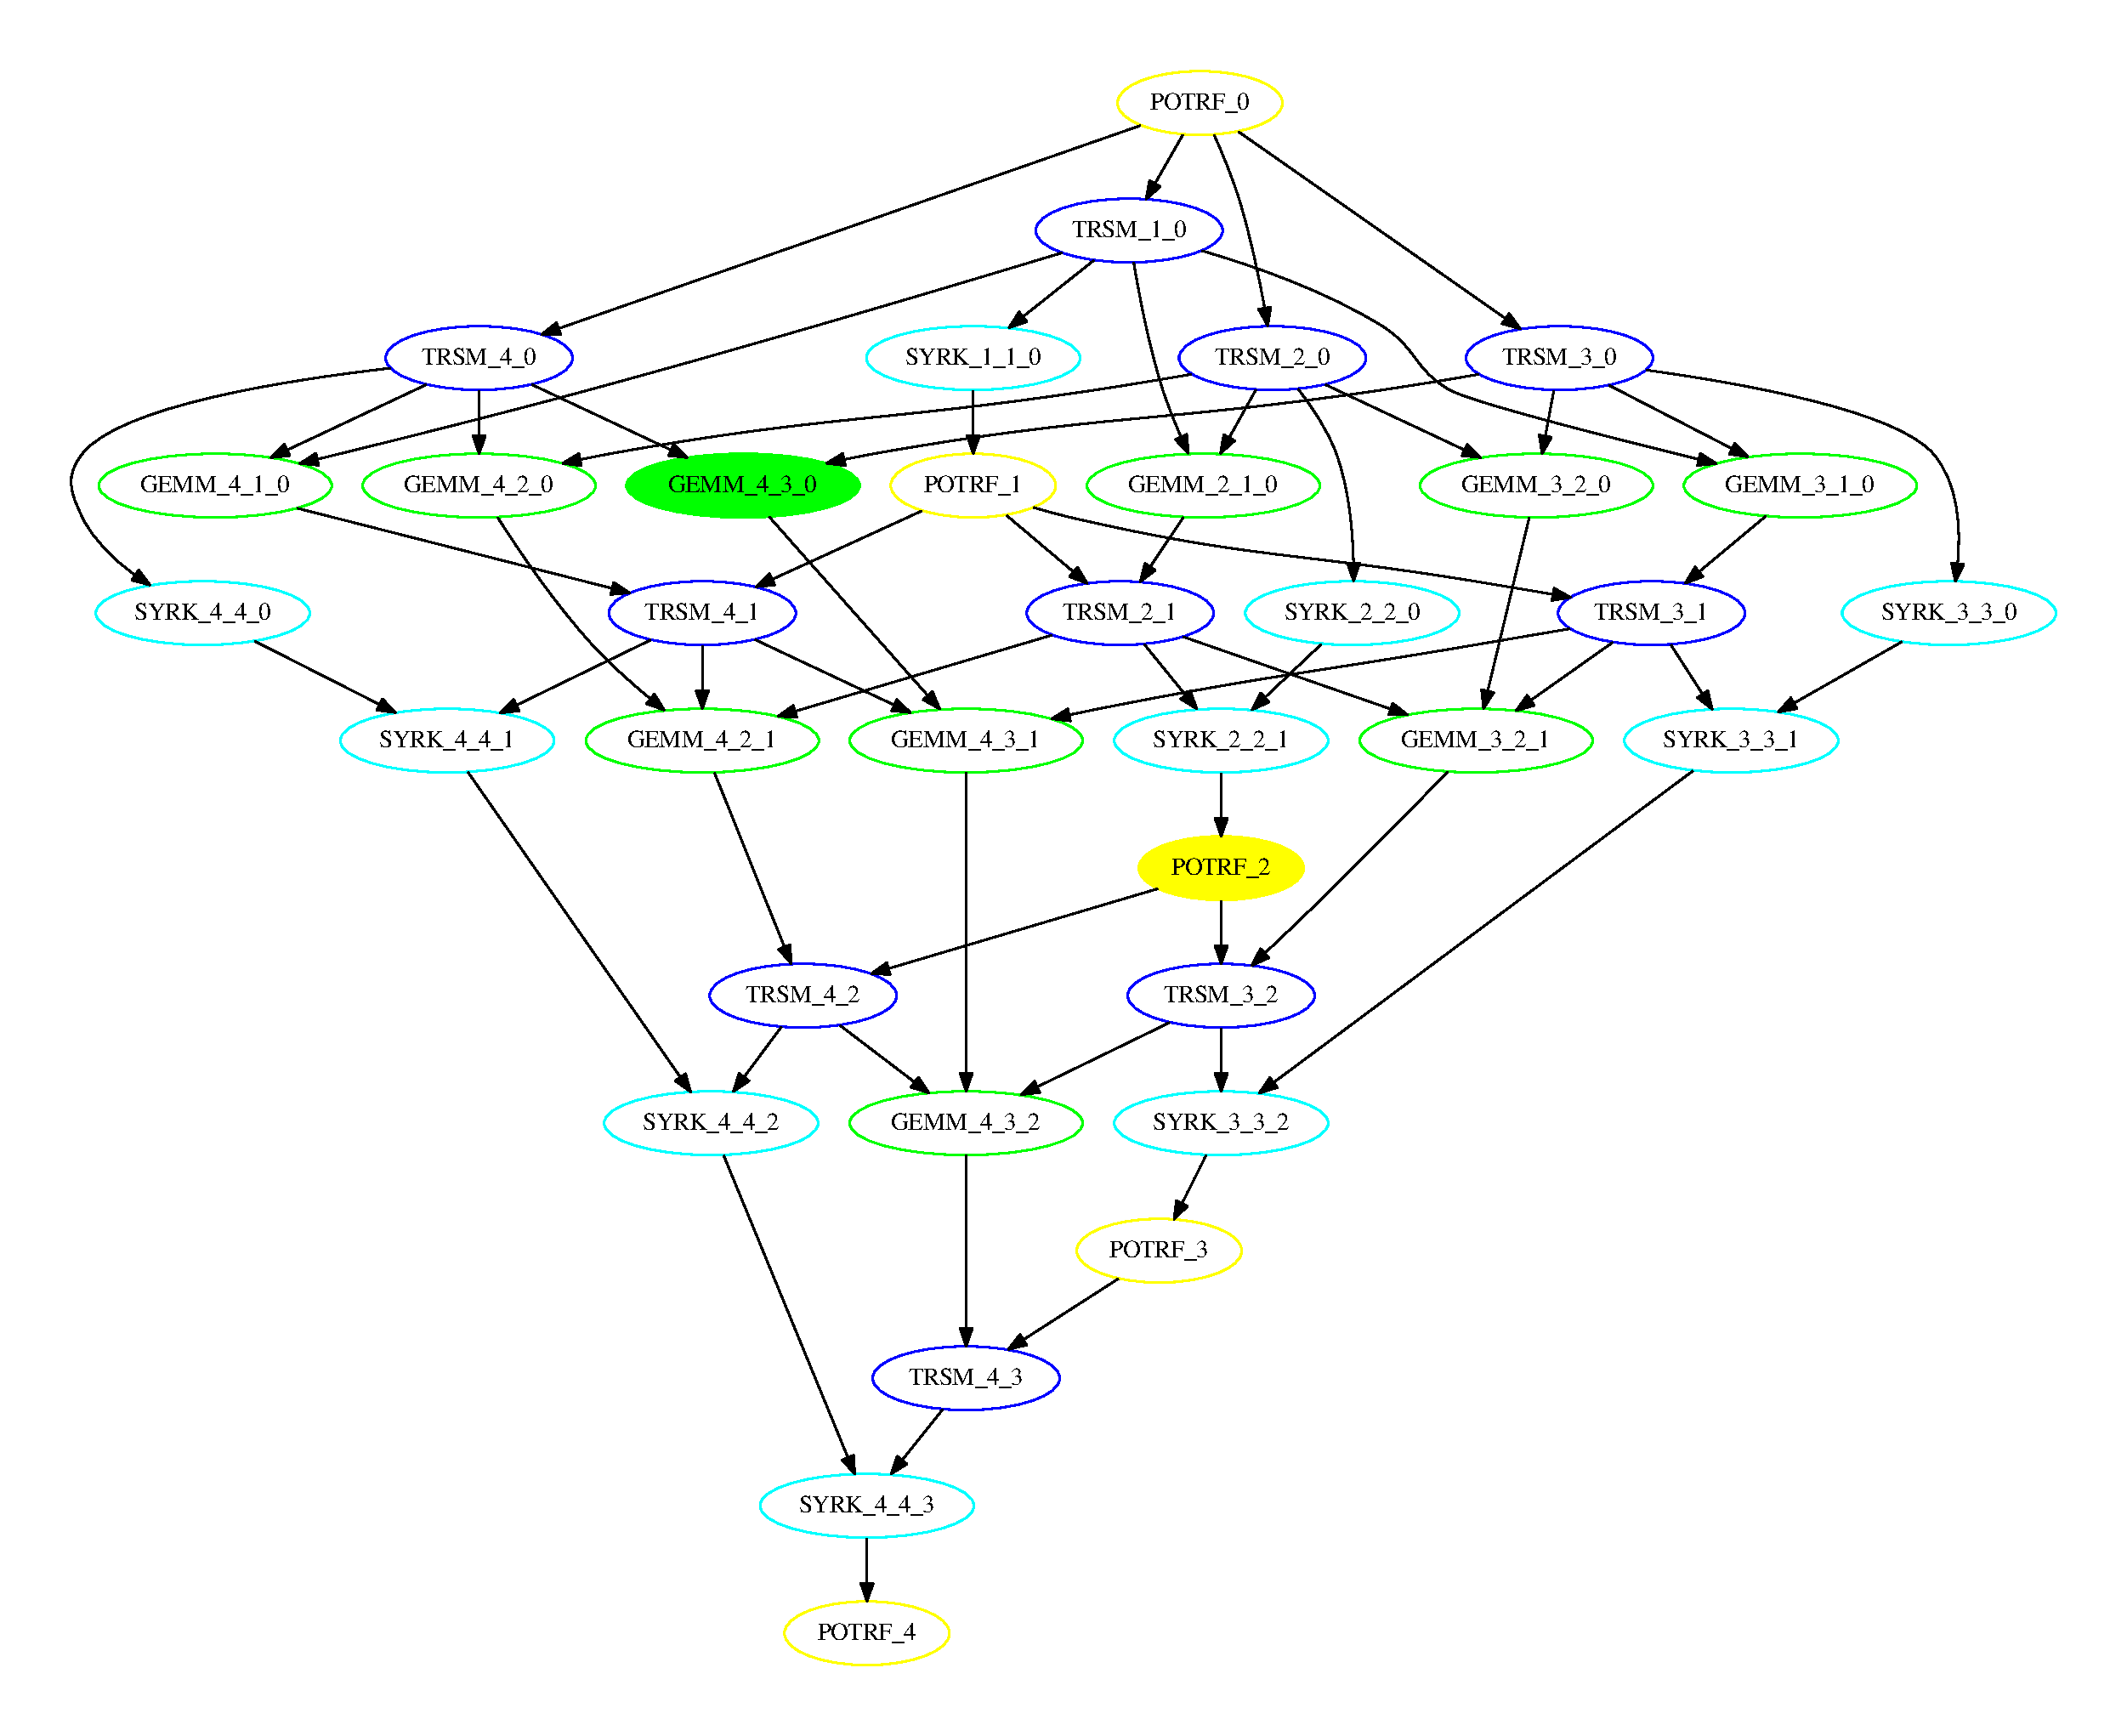
\includegraphics[scale=0.20]{./diagrams/cholesky_TwoNodesHighlighted_5.pdf}
		%%		\includegraphics[scale=0.20]{figs/CholeskyTaskGraphs/test2.pdf}
		%  \end{block}
	\end{figure}
	{\footnotesize
		\begin{itemize}
			\item Does not need synchronization at each outer iteration
			%%		\item Exhibits complex dependencies pattern
		\end{itemize}
	}
	
\end{frame}



\begin{frame}{Performance vs Bounds of Cholesky Factorization}
\framesubtitle{With StarPU {\it dmdas} (HEFT based) scheduler on a single node}
\begin{center}
	\includegraphics[scale=0.8]{./diagrams/Actual_vs_GEMMBound.eps}
	
	{
		%			\textcolor{blue}{$\bullet$} 
		Gap between performance and bound is significant
	}
\end{center}
\end{frame}

\begin{frame}{Our Contributions --  Single Node Perspective}
\begin{itemize}
	\item Better bounds on performance
	\vfill
	%%	\item Static vs Dynamic strategies
	%%	\begin{itemize}
	%%		\item Inject static knowledge into dynamic schedulers
	%%		\item Inject dynamic corrections into static scheduler
	%%	\end{itemize}
	%%	\vfill
	\item A resource centric \heteroprio scheduler for task graphs on two types of resources
	\vfill
	\item Performance guarantee of \heteroprio for a set of independent tasks on two types of resources   
\end{itemize}
\end{frame}

\begin{frame}{Machine Information \& Library used}
\begin{itemize}
	\item Cholesky kernel of Chameleon library with StarPU runtime 
	\item We use TileSize (BlockSize) =960
	\item Heterogeneous platform description (Single Node)
	\begin{itemize}
		\item 12 CPU cores (\textbf{9 computational cores}) of Intel R Xeon R X5650 processors
		\item \textbf{3} Nvidia Tesla M2070 \textbf{GPUs}
		\item Theoretical peak performance = 1641 GFlop/s 
		\item GEMM peak performance = 981 GFlop/s   
		\begin{table}[htb]
			\label{table:gpus_performance}
			\begin{center}
				
				\begin{tabular}{|c|c|c|c|} \hline POTRF & TRSM & SYRK & GEMM \\
					\hline $\simeq$2$\times$ & $\simeq$11$\times$ & $\simeq$26$\times$ &
					$\simeq$29$\times$ \\ \hline
				\end{tabular}  
				\caption{GPUs relative performance}
			\end{center}
		\end{table}
	\end{itemize}
\end{itemize}
\end{frame}

%%\begin{frame}{Framework}
%%\begin{block}{\centering {\scriptsize Actual Execution}}
%%	\centering \includegraphics[width=0.8\linewidth]{framework/Actual_execution}
%%\end{block}
%%\only<2>
%%{
%%	\begin{center}
%%		\begin{itemize}
%%			\item Real-life experimentation poses problems
%%			\begin{itemize}
%%				\item Platform unavailability
%%				\item Unexpected software upgrades
%%				\item Irreproducible behavior
%%			\end{itemize}
%%		\end{itemize}
%%	\end{center}
%%}
%%\end{frame}
%%
%%\begin{frame}{Proposed Framework}
%%\begin{center}
%%\begin{block}{\centering {\scriptsize Simulation}}
%%	%  \begin{columns}
%%	%     \begin{column}[c]{.5\linewidth}
%%	%      \begin{itemize}
%%	%       \item {\scriptsize Truly reproducible experiments}
%%	%       \item {\scriptsize Can even tune the platform}
%%	%       \begin{itemize}
%%	%	\item[-] {\scriptsize e.g. change number of CPUs/GPUs}
%%	%	\end{itemize}
%%	%      \end{itemize}
%%	%  \end{column}
%%	%  \begin{column}[c]{.5\linewidth}
%%	%%    \begin{block}
%%	%   \centering \includegraphics[height=2.4 cm, 
%%	%width=0.94\linewidth]{framework/Simulation}
%%	%%    \end{block}
%%	%  \end{column}
%%	%
%%	% \end{columns}
%%	\centering \includegraphics[height=2.24 cm]{framework/Simulation}
%%\end{block}
%%\begin{itemize}
%%	\item {\scriptsize Truly reproducible experiments}
%%	\item {\scriptsize Can even tune the platform 
%%		e.g. change number of CPUs/GPUs}
%%\end{itemize}
%%
%%\begin{block}{\centering {\scriptsize Simulation without communication cost}}
%%	%  \begin{columns}
%%	%    \begin{column}[c]{.5\linewidth}
%%	%   \centering \includegraphics[height=2.4 cm]{framework/Simulation_nocomm}
%%	%  \end{column}
%%	%     \begin{column}[c]{.5\linewidth}
%%	%      \begin{itemize}
%%	%       \item {\scriptsize To simplify scheduling problem}
%%	%       \begin{itemize}
%%	%        \item {\scriptsize Don't consider communication cost}
%%	%       \end{itemize}
%%	%      \end{itemize}
%%	%  \end{column}
%%	% \end{columns}
%%	\centering \includegraphics[height=2.24 cm]{framework/Simulation_nocomm}
%%\end{block}
%%\begin{itemize}
%%	\item {\scriptsize To simplify scheduling problem -- Don't consider 
%%		communication cost}
%%\end{itemize}
%%\end{center}
%%
%%\end{frame}



\begin{frame}{Impact of communication on Cholesky Factorization}
\framesubtitle{With StarPU {\it dmdas} (HEFT based) scheduler}
\includegraphics[scale=0.8]{./diagrams/Actual_vs_Simgrid_vsSimgridnocomm}

\scriptsize{Impact of communication on performance is very less for larger matrices}
\end{frame}





\subsubsection{Task Graph Bound}
\begin{frame}{Area Bound}
\begin{columns}
	\begin{column}[c]{.5\linewidth}
		\begin{block}{\centering {\scriptsize DAG}}
			\centering \includegraphics[scale=0.25]{boundsDiagram/taskgraph}
		\end{block}
	\end{column}
	
	\begin{column}[c]{.5\linewidth}
		\begin{block}{\centering {\scriptsize No Dependencies}}
			\centering \includegraphics[scale=0.25]{boundsDiagram/taskgraphNoDep}
		\end{block}
	\end{column}
\end{columns}
\begin{block}{\centering {\scriptsize Minimum execution time (minimize \textit{l})}}
	\centering \includegraphics[scale=0.45]{boundsDiagram/schedule}
\end{block}

\end{frame}



\begin{frame}{Iterative Bound}
\begin{columns}
	\begin{column}[c]{.5\linewidth}
		\begin{block}{\centering {\scriptsize DAG}}
			\only<1-3> {\centering \includegraphics[scale=0.25]{boundsDiagram/taskgraph}}
			%\only<2-3> {\centering 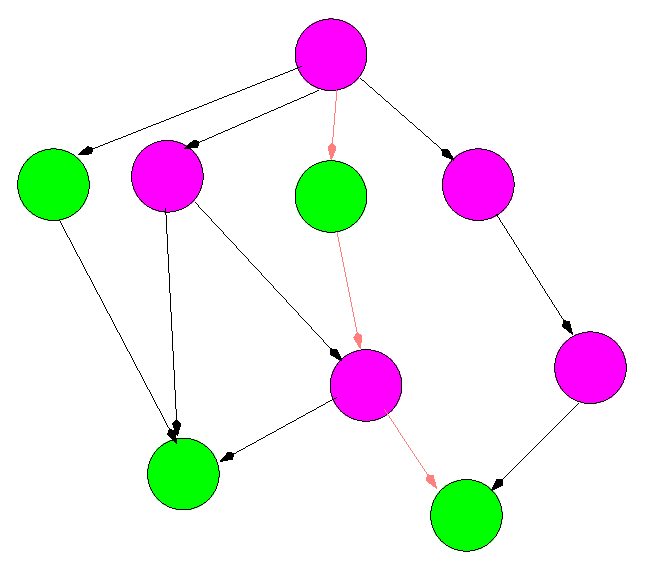
\includegraphics[scale=0.25]{boundsDiagram/taskgraphPath}}
		\end{block}
	\end{column}
	
	\begin{column}[c]{.5\linewidth}
		\begin{block}{\centering {\scriptsize \only<1> {No} \only<2-3> {Some} 
					Dependencies}}
			\only<1> {\centering \includegraphics[scale=0.25]{boundsDiagram/taskgraphNoDep}}
			\only<2-3> {\centering \includegraphics[scale=0.25]{boundsDiagram/taskgraphOnePath}}
		\end{block}
	\end{column}
\end{columns}
\begin{block}{\centering {\scriptsize Minimum execution time (minimize \textit{l})}}
	\begin{columns}
		\begin{column}[c]{.5\linewidth}
			\centering \includegraphics[scale=0.45]{boundsDiagram/schedule}   
		\end{column}
		\begin{column}[c]{.5\linewidth}
			\only<2-3>
			{
				\begin{itemize}
					\item[$\star$]{\scriptsize If any path in DAG is larger than \textit{l}}
					\only<3>{
						\begin{itemize}
							\item {\scriptsize add this path as a constraint and repeat the procedure}
						\end{itemize}
					}
				\end{itemize}
			}
			
		\end{column}  
	\end{columns}
\end{block}

\end{frame}

\begin{frame}{Comparison of Simulated Performance and Bounds}
\begin{center}
	\includegraphics[scale=0.8]{./diagrams/boundsVsSimulation}
\end{center}
\end{frame}

\subsubsection{Dynamic Scheduling Strategies}
\begin{frame}{Dynamic Scheduling}
\begin{itemize} 
	\item Decide based on state of resources and estimation of 
	execution/transfer time
	\item Possibly uses some priorities among the ready tasks
	\item Pros: Fault tolerance, Load balancing
	\item Cons: may be less efficient due to local views
\end{itemize}
\end{frame}

\begin{frame}{heft scheduler}
\begin{itemize}
	\item Task centric scheduler
	%\item Based on minimum completion time (MCT) heuristic 
	\item Based on Heterogeneous Early Finish time (HEFT) heuristic (proposed by \textit{Topcuoglu et al.} in 2002)
	%\item Similar to StarPU dmdas scheduler
\end{itemize}
\begin{block}{}
	\begin{columns}
		\begin{column}[c]{.5\linewidth}
			\begin{itemize}
				\item $A$ is highest priority ready task at $t$ 
				\item Completion time on resource2 is minimum
				\item Task $A$ schedules on resource2
			\end{itemize}
			
		\end{column}
		\begin{column}[c]{.5\linewidth}
			\centering \includegraphics[scale=0.45]{basicSchedulers/heftp1} 
			
			\centering \includegraphics[scale=0.45]{basicSchedulers/heftp2}
		\end{column}
		
	\end{columns}
	
\end{block}

\end{frame}


\begin{frame}{heft  Scheduler}
\framesubtitle{heft trace for 12 X 12  blocks of Cholesky Factorization}
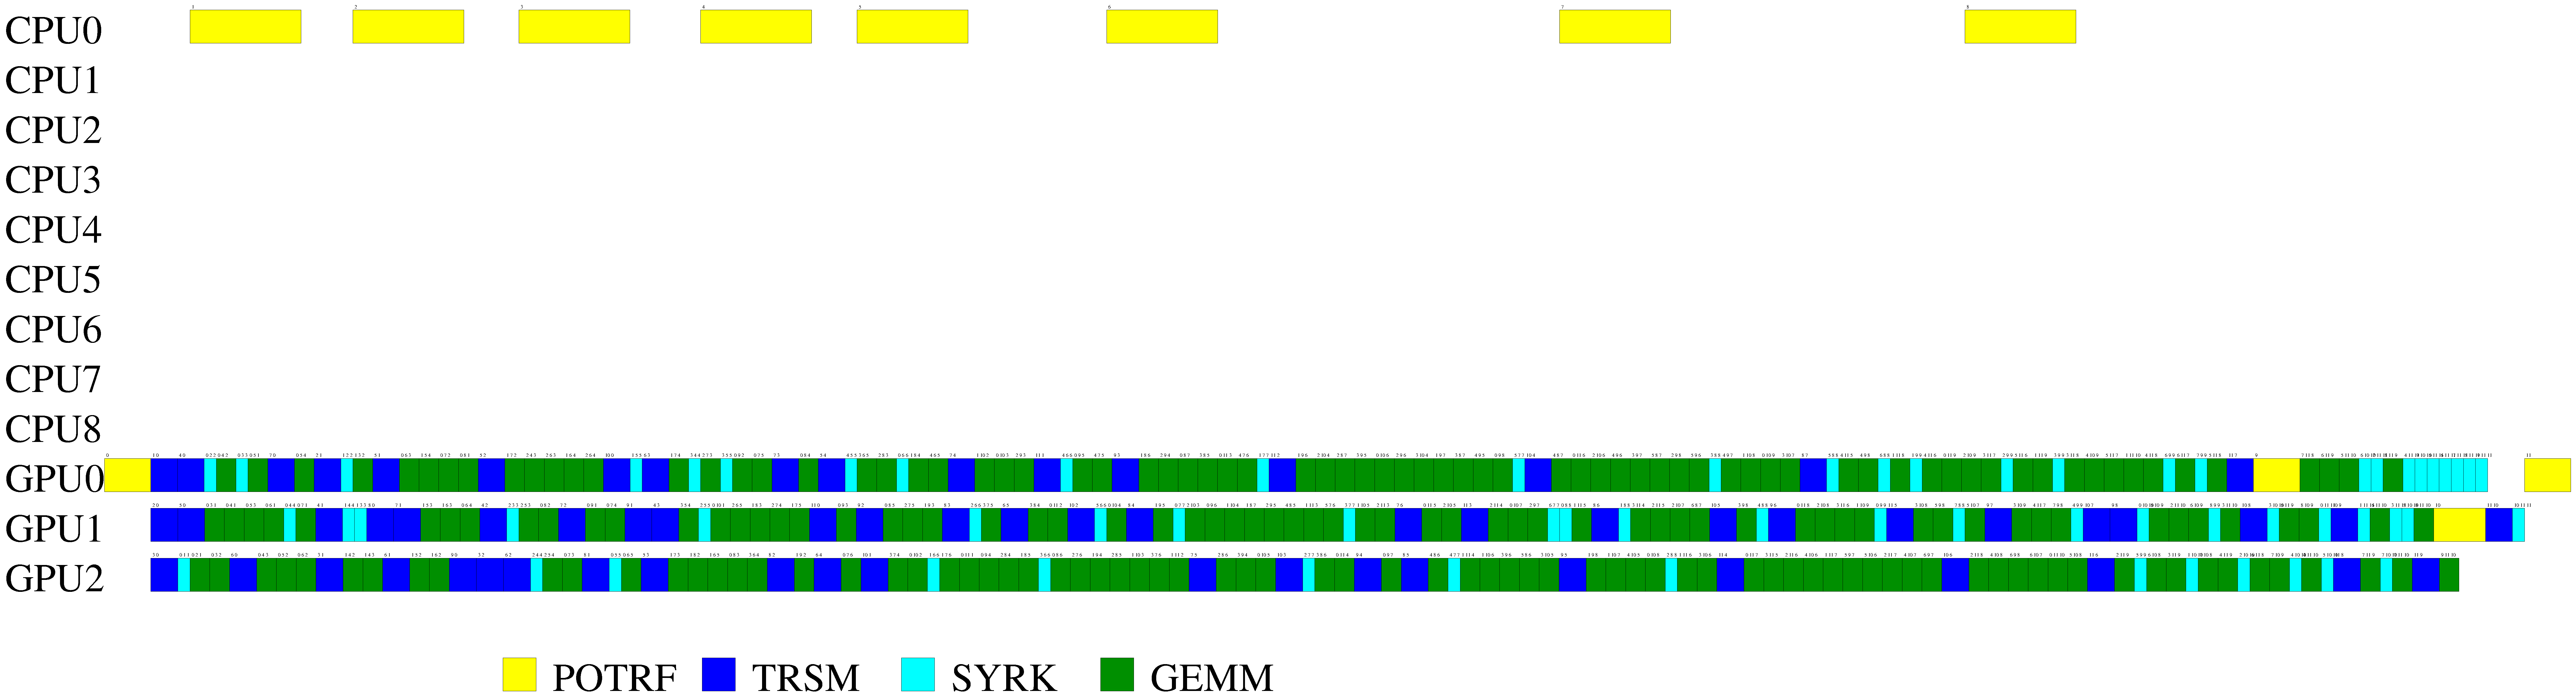
\includegraphics[width=\textwidth,height=0.75\textheight]{./diagrams/heftp-12}
\begin{itemize}
\item Most of the CPU resources are not utilized (686 GFlop/s)
%%\item SS performance = 791 GFlop/s
\end{itemize}
\end{frame}


\begin{frame}{\heteroprio (HP) Scheduler}
\begin{itemize}
	\item Resource centric scheduler
	\item Based on tasks heterogeneity factors   
	\item Proposed by \textit{Agullo et al.} in 2016 for a large set of small independent tasks 
\end{itemize}
\begin{block}{}
	\begin{columns}
		\begin{column}[c]{.4\linewidth}
			\begin{itemize}
				\item {\scriptsize $A$ is highest priority ready task at $t$} 
				\item {\scriptsize Resource1 is best suited to task $C$}
				\item {\scriptsize Resource1 selects task $C$}
			\end{itemize}
			
		\end{column}
		\begin{column}[c]{.6\linewidth}
			\centering \includegraphics[scale=0.45]{basicSchedulers/heteroprio1} 
			
			\centering \includegraphics[scale=0.45]{basicSchedulers/heteroprio2}
		\end{column}
		
	\end{columns}
	
\end{block}

\end{frame}

\begin{frame}{HP scheduler}
\framesubtitle{HP trace for 12 X 12  blocks of Cholesky Factorization}
%% \includegraphics[width=\textwidth,height=0.75\textheight]{fig-GP-2016/heteroprio-12}
\includegraphics[width=\textwidth,height=0.5\textheight]{./diagrams/heteroprio-12}
\begin{itemize}
\item Not much emphasis on progress (431 GFlop/s)
%%\item SS performance = 791 GFlop/s
%%\item Best heft variant performance = 726 GFlop/s 
%% \item Iterative Bound = 836 GFlop/s
\end{itemize}
\end{frame}


\begin{frame}{\heteroprio (HP) with spoliation (SP)}
\begin{itemize}
	\item HP scheduler
	\begin{itemize}
		\item Good CPU Utilization
		\item Ignorance of critical path
		\item Significant idle time on GPUs
	\end{itemize}
	\item HP with spoliation (HP+SP)
	\begin{itemize}
		\item  An idle GPU restarts highest priority CPU task if it finishes earlier
	\end{itemize}
\end{itemize}
\end{frame}


\begin{frame}{Successive correction to HP+SP with static information}
%  \begin{itemize}
%   \item Combined ready queues view for GPUs (HP+CGV)
%   \item Potrf preemption on CPU (HP+PP)
%   \item Priority constraints on CPU tasks (HP+PC)
%   \begin{itemize}
%    \item POTRF tasks are relaxed (HP+PCEP)
%    \item POTRF \& TRSM tasks are relaxed (HP+PCEPT)
%   \end{itemize}
% 
%  \end{itemize}

$\bullet$CPU selects lowest 
priority task among all tasks of 
same acceleration factor -- \textbf{NonBlocking} \\ 
$\bullet$\textcolor{orange}{HP+CGV}: GPU selects highest 
priority task among all tasks of 
similar acceleration factors -- \textbf{Progress} \\

$\bullet$\textcolor{orange}{HP+PP}: \textcolor{yellow}{POTRF} preempted on CPU (less accelerated on GPU) -- \textbf{Best Affinity} \\
$\bullet$\textcolor{orange}{HP+PCEPT}: GPU restarts highest 
priority \textcolor{green}{GEMM}/\textcolor{cyan}{SYRK} task if 
it finishes earlier -- \textbf{NonBlocking} 
%  431.45 722.85 759.99
\end{frame}


\begin{frame}{HP+PCEPT scheduler}
\framesubtitle{HP+PCEPT trace for 12 X 12  blocks of Cholesky Factorization}
% 
% \begin{itemize}
%  \item Achieved performance = 759.99 GFLop/s
% \end{itemize}

\only<1>{\includegraphics[width=\textwidth,height=0.75\textheight]{./diagrams/heteroprio+PCEPT-12}}
\only<2>{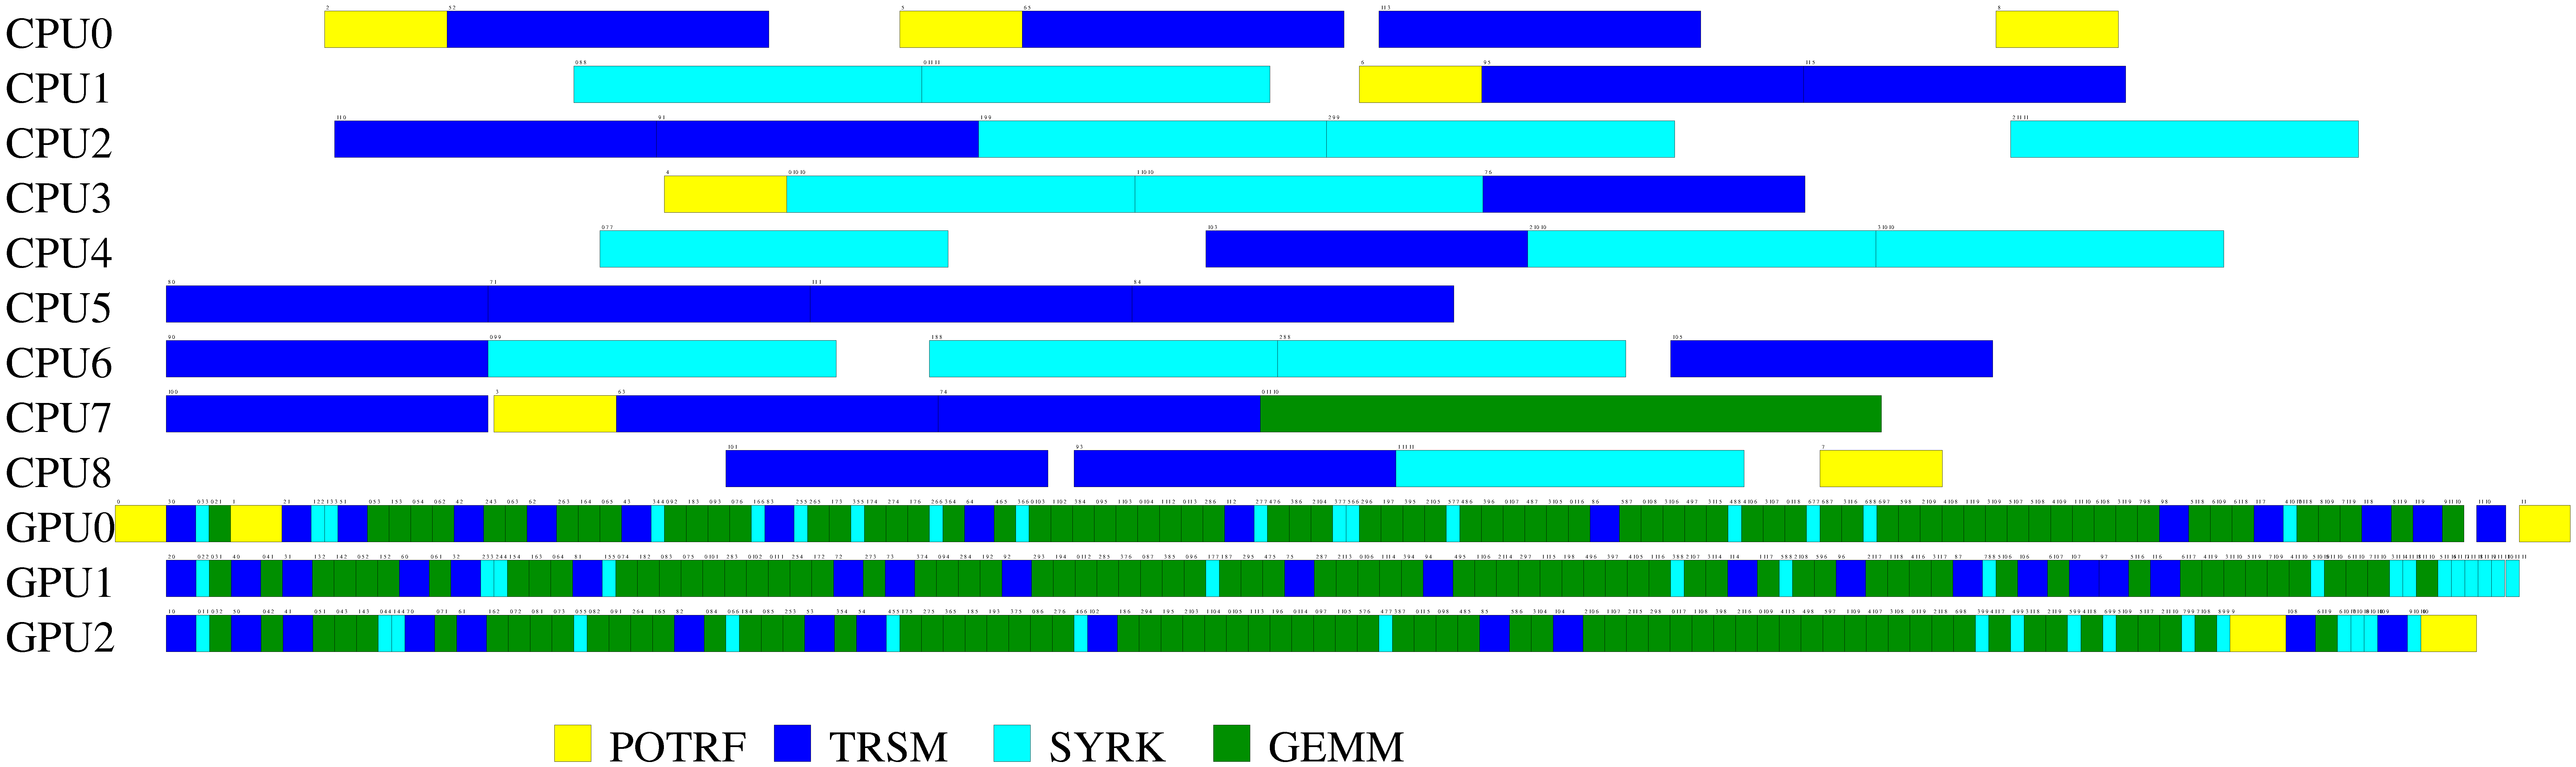
\includegraphics[width=\textwidth,height=0.75\textheight]{./diagrams/HP+PCEPTWithoutAbortedTasks}}

Achieved performance = 760 GFLop/s \\
{\small heft best performance = 726 GFlop/s}
\end{frame}


\begin{frame}{SS-Vs-heft-Vs-HP-Vs-Bound}
\begin{center}
	\includegraphics[scale=0.8]{./diagrams/bestVariantsWithBound}
\end{center}
\end{frame}


\begin{frame}{Actual execution trace for 12 X 12  blocks  of Cholesky Factorization}
\heteroprio schedule with 5\% increase in CPU execution timings
\begin{center}
	\includegraphics[scale=0.65]{./diagrams/paje-12-5-withResources}
\end{center}
\end{frame}


\begin{frame}{\heteroprio Approximation Ratios and Worst Case Example Ratios}
\begin{center}
	\begin{tabular}{|c|c|c|}
		\hline
		(\#CPUs, \#GPUs) & Approximation ratio & Worst case ex. \\ 
		\hline
		(1,1) & $\frac{1 + \sqrt{5}}{2}$ & $\frac{1 + \sqrt{5}}{2}$\\ \hline
		%			(1,n) & $2$ \\ \hline
		(m,1) & $\frac{3 + \sqrt{5}}{2}$ & $\frac{3 + \sqrt{5}}{2}$\\ \hline
		%			(m,n) \& $m \le n-1$ & $3$ \\ \hline
		%			(m,n) & $2 + \sqrt{2} \approx 3.41 $ &  $3$\\ \hline
		(m,n) & $2 + \sqrt{2} \approx 3.41 $ & $2 +
		\frac{2}{\sqrt{3}} \approx 3.15$\\ \hline
	\end{tabular}
\end{center}
\end{frame}



\begin{frame}{1 CPU 1 GPU \heteroprio Worst Case Example}

\begin{block}{}
	\begin{center}
		\begin{tabular}{|c|c|c|c|}
			\hline
			Task & CPU Time & GPU Time & accel ratio \\ \hline
			$X$ & $\phi$ & $1$ & $\phi$ \\ \hline
			$Y$ & $1$ & $\frac{1}{\phi}$ & $\phi$ \\ \hline 
		\end{tabular}
		%			\begin{flushleft}
		\\ \hspace*{-5 cm}	Where $\phi = \frac{1+\sqrt{5}}{2}$ 
		%			\end{flushleft}
	\end{center}
	%%		Two tasks $X$ and $Y$, with $p_X = \phi$, $q_X = 1$, $p_Y = 1$ and $q_Y = \frac{1}{\phi}$ such that $\rho_X = \rho_Y = \phi$
\end{block}
\begin{figure}
	\begin{columns}
		\begin{column}{0.45\linewidth}
			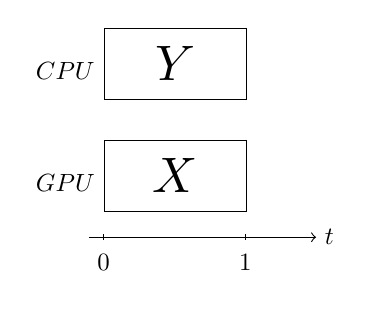
\begin{tikzpicture}[decoration={brace, amplitude=5},scale=1.8, every node/.style={scale=1.8}]
			\node(t1) at (0,0) {};       		
			\node[above right=0cm and 0cm of t1.mid, draw, minimum height=0.5cm, minimum width=1cm,draw,fill=white](t2) {$X$};
			
			\node[above right=0.5cm and 0cm of t2.north west, draw, minimum height=0.5cm, minimum width=1cm,draw,fill=white](t3) {$Y$};			
			
			\node[above left=0.15cm and 0cm of t2.south west, scale=0.5, rotate=0] {$GPU$};
			\node[above left=0.15cm and 0cm of t3.south west, scale=0.5, rotate=0] {$CPU$};		
			
			\tikzstyle{legend}=[below=0.35, anchor=mid] 	
			\draw[->] (-0.1, -0.1) -- (0, -0.1)  node[legend,scale=0.5] {$0$} --(1,-0.1) node [legend,scale=0.5] {$1$} --(1.5, -0.1) node[right,scale=0.5] {$t$}; 
			
			\foreach \x in {0cm, 1cm} \draw (\x, -0.12) -- (\x, -0.08);
			%%			To align both figures of subfloat-- an object without drawing at the same depth
			\path (-0.1, -0.5) -- (1.5, -0.5);
			
			\end{tikzpicture}
			\caption{Optimal schedule}
		\end{column}
		\begin{column}{0.4\linewidth}
			\begin{tikzpicture}[decoration={brace, amplitude=5},scale=1.8, every node/.style={scale=1.8}]
			\node(t1) at (0,0) {};      		
			
			\node[above right=0cm and 0cm of t1.mid, draw, minimum height=0.5cm, minimum width=0.618cm,draw,fill=white](t2) {$Y$};
			
			\node[above right=0.5cm and 0cm of t2.north west, draw, minimum height=0.5cm, minimum width=1.618cm,draw,fill=white](t3) {$X$};								
			
			\tikzstyle{legend}=[below=0.35, anchor=mid] 	
			\draw[->] (-0.1, -0.1) -- (0, -0.1)  node[legend,scale=0.5] {$0$} --(0.618,-0.1) node [legend,scale=0.5] {$\tfrac{1}{\phi}$} --(1.618,-0.1) node [legend,scale=0.5] {$\phi$} --(2, -0.1) node[right,scale=0.5] {$t$}; 
			
			\foreach \x in {0cm, 0.618cm, 1.618cm} \draw (\x, -0.12) -- (\x, -0.08);
			%%			To align both figures of subfloat -- an object without drawing at the same depth
			
			\path (-0.1, -0.5) -- (2, -0.5);
			
			\end{tikzpicture}
			\caption{\heteroprio schedule}
		\end{column}		
	\end{columns}
\end{figure}
\end{frame}	


%%\begin{frame}{Schedulers}
%%content...
%%\end{frame}
%%\begin{frame}{HeteroPrio}
%%content...
%%\end{frame}
%%\begin{frame}{Performance Results with \heteroprio}
%%content...
%%\end{frame}
%%\begin{frame}{Approximation Ratio of \heteroprio}
%%content...
%%\end{frame}
%%\begin{frame}{Worst Case Examples}
%%content...
%%\end{frame}

\part[Proposed Plan]{Part2}
\begin{frame}
\frametitle{Overview} % Table of contents slide, comment this block out to remove it
\tableofcontents[part=2] % Throughout your presentation, if you choose to use \section{} and \subsection{} commands, these will automatically be printed on this slide as an overview of your presentation
\end{frame}
\section{Modify Existing Algorithms}
\begin{frame}{Modify Existing Algorithms}
\begin{itemize}
	\item Understand the existing Algorithms
	\item Derive communication lower bounds 
	\item Design new algorithms \& implement them
	\item Homogeneous Systems
	\item Extend the same principle for Heterogeneous Systems
\end{itemize}
\end{frame}
\setcounter{section}{20}
\subsection{Extension of the Existing Approaches}
\begin{frame}{Tensor Contraction \& Strassen's Matrix Multiplication}
content...
\end{frame}
\begin{frame}{Hierarchical Matrix concepts to Tensors}
content...
\end{frame}
\begin{frame}{Roofline model with Dependencies}
content...
\end{frame}
\subsection{Exploratory Topics}
\begin{frame}{New Tensor Representations}
content...
\end{frame}
\begin{frame}{Architecture Aware Algorithms}
content...
\end{frame}
\begin{frame}{Randomization in Tensor Computations}
content...
\end{frame}
\section{Integration in the Team}
\begin{frame}{Integration in the Team}
content...
\end{frame}

%%%%%----------------------------------------------------------------------------------------
%%%%%	PRESENTATION SLIDES
%%%%%----------------------------------------------------------------------------------------
%%%%
%%%%%------------------------------------------------
%%%%\section{First Section} % Sections can be created in order to organize your presentation into discrete blocks, all sections and subsections are automatically printed in the table of contents as an overview of the talk
%%%%%------------------------------------------------
%%%%
%%%%\subsection{Subsection Example} % A subsection can be created just before a set of slides with a common theme to further break down your presentation into chunks
%%
%%\begin{frame}
%%\frametitle{Paragraphs of Text}
%%Sed iaculis dapibus gravida. Morbi sed tortor erat, nec interdum arcu. Sed id lorem lectus. Quisque viverra augue id sem ornare non aliquam nibh tristique. Aenean in ligula nisl. Nulla sed tellus ipsum. Donec vestibulum ligula non lorem vulputate fermentum accumsan neque mollis.\\~\\
%%
%%Sed diam enim, sagittis nec condimentum sit amet, ullamcorper sit amet libero. Aliquam vel dui orci, a porta odio. Nullam id suscipit ipsum. Aenean lobortis commodo sem, ut commodo leo gravida vitae. Pellentesque vehicula ante iaculis arcu pretium rutrum eget sit amet purus. Integer ornare nulla quis neque ultrices lobortis. Vestibulum ultrices tincidunt libero, quis commodo erat ullamcorper id.
%%\end{frame}
%%
%%%------------------------------------------------
%%
%%\begin{frame}
%%\frametitle{Bullet Points}
%%\begin{itemize}
%%\item Lorem ipsum dolor sit amet, consectetur adipiscing elit
%%\item Aliquam blandit faucibus nisi, sit amet dapibus enim tempus eu
%%\item Nulla commodo, erat quis gravida posuere, elit lacus lobortis est, quis porttitor odio mauris at libero
%%\item Nam cursus est eget velit posuere pellentesque
%%\item Vestibulum faucibus velit a augue condimentum quis convallis nulla gravida
%%\end{itemize}
%%\end{frame}
%%
%%%------------------------------------------------
%%
%%\begin{frame}
%%\frametitle{Blocks of Highlighted Text}
%%\begin{block}{Block 1}
%%Lorem ipsum dolor sit amet, consectetur adipiscing elit. Integer lectus nisl, ultricies in feugiat rutrum, porttitor sit amet augue. Aliquam ut tortor mauris. Sed volutpat ante purus, quis accumsan dolor.
%%\end{block}
%%
%%\begin{block}{Block 2}
%%Pellentesque sed tellus purus. Class aptent taciti sociosqu ad litora torquent per conubia nostra, per inceptos himenaeos. Vestibulum quis magna at risus dictum tempor eu vitae velit.
%%\end{block}
%%
%%\begin{block}{Block 3}
%%Suspendisse tincidunt sagittis gravida. Curabitur condimentum, enim sed venenatis rutrum, ipsum neque consectetur orci, sed blandit justo nisi ac lacus.
%%\end{block}
%%\end{frame}
%%
%%%------------------------------------------------
%%
%%\begin{frame}
%%\frametitle{Multiple Columns}
%%\begin{columns}[c] % The "c" option specifies centered vertical alignment while the "t" option is used for top vertical alignment
%%
%%\column{.45\textwidth} % Left column and width
%%\textbf{Heading}
%%\begin{enumerate}
%%\item Statement
%%\item Explanation
%%\item Example
%%\end{enumerate}
%%
%%\column{.5\textwidth} % Right column and width
%%Lorem ipsum dolor sit amet, consectetur adipiscing elit. Integer lectus nisl, ultricies in feugiat rutrum, porttitor sit amet augue. Aliquam ut tortor mauris. Sed volutpat ante purus, quis accumsan dolor.
%%
%%\end{columns}
%%\end{frame}
%%
%%%------------------------------------------------
%%\section{Second Section}
%%%------------------------------------------------
%%
%%\begin{frame}
%%\frametitle{Table}
%%\begin{table}
%%\begin{tabular}{l l l}
%%\toprule
%%\textbf{Treatments} & \textbf{Response 1} & \textbf{Response 2}\\
%%\midrule
%%Treatment 1 & 0.0003262 & 0.562 \\
%%Treatment 2 & 0.0015681 & 0.910 \\
%%Treatment 3 & 0.0009271 & 0.296 \\
%%\bottomrule
%%\end{tabular}
%%\caption{Table caption}
%%\end{table}
%%\end{frame}
%%
%%%------------------------------------------------
%%
%%\begin{frame}
%%\frametitle{Theorem}
%%\begin{theorem}[Mass--energy equivalence]
%%$E = mc^2$
%%\end{theorem}
%%\end{frame}
%%
%%%------------------------------------------------
%%
%%\begin{frame}[fragile] % Need to use the fragile option when verbatim is used in the slide
%%\frametitle{Verbatim}
%%\begin{example}[Theorem Slide Code]
%%\begin{verbatim}
%%\begin{frame}
%%\frametitle{Theorem}
%%\begin{theorem}[Mass--energy equivalence]
%%$E = mc^2$
%%\end{theorem}
%%\end{frame}\end{verbatim}
%%\end{example}
%%\end{frame}
%%
%%%------------------------------------------------
%%
%%\begin{frame}
%%\frametitle{Figure}
%%Uncomment the code on this slide to include your own image from the same directory as the template .TeX file.
%%%\begin{figure}
%%%\includegraphics[width=0.8\linewidth]{test}
%%%\end{figure}
%%\end{frame}
%%
%%%------------------------------------------------
%%
%%\begin{frame}[fragile] % Need to use the fragile option when verbatim is used in the slide
%%\frametitle{Citation}
%%An example of the \verb|\cite| command to cite within the presentation:\\~
%%
%%This statement requires citation \cite{p1}.
%%\end{frame}
%%
%%%------------------------------------------------
%%
%%\begin{frame}
%%\frametitle{References}
%%\footnotesize{
%%\begin{thebibliography}{99} % Beamer does not support BibTeX so references must be inserted manually as below
%%\bibitem[Smith, 2012]{p1} John Smith (2012)
%%\newblock Title of the publication
%%\newblock \emph{Journal Name} 12(3), 45 -- 678.
%%\end{thebibliography}
%%}
%%\end{frame}
%%
%%%------------------------------------------------
%%
%%\begin{frame}
%%\Huge{\centerline{The End}}
%%\end{frame}

%----------------------------------------------------------------------------------------

\end{document} 